%%%%%%%%%%%%%%%%%%%%%%%%%%%%% Thesis.tex %%%%%%%%%%%%%%%%%%%%%%%%%%%%%%%
%                                                                      %
%  ---------- Master of Science Dissertation template ----------       %
%                                                                      %
%  Template for the Master Thesis according to the regulations         %
%  published by the Academic Board (Direcção Académica) at IST.        %
%                                                                      %
%  For up-to-date guide, please refer to the official website          %
%  http://academica.tecnico.ulisboa.pt/alunos/dissertacao-de-mestrado/ %
%                                                                      %
%       Andre C. Marta                                                 %
%       Area Cientifica de Mecanica Aplicada e Aeroespacial            %
%       Departamento de Engenharia Mecanica                            %
%       Instituto Superior Tecnico                                     %
%       Av. Rovisco Pais                                               %
%       1049-001 Lisboa                                                %
%       Portugal                                                       %
%       Tel: +351 21 841 9469                                          %
%                        3469 (extension)                              %
%       Email: andre.marta@tecnico.ulisboa.pt                          %
%                                                                      %
%  Created:       Jan 20, 2011                                         %
%  Last Modified: Feb 19, 2018                                         %
%                                                                      %
%%%%%%%%%%%%%%%%%%%%%%%%%%%%%%%%%%%%%%%%%%%%%%%%%%%%%%%%%%%%%%%%%%%%%%%%
%  Revision history                                                    %
%  v1 - 2011/01/24 - original template                                 %
%  v2 - 2012/10/30 - new IST image and glossary support                %
%  v3 - 2013/12/10 - update according to 2012/13 official guide        %
%  v4 - 2014/02/28 - new default for bibliography style                %
%  v5 - 2014/05/07 - update according to 2013/14 official guide        %
%  v6 - 2015/07/02 - cover page format fixed,                          %
%                    contents page numbering fixed,                    %
%                    better language support,                          %
%                    enhanced examples of tables,                      %
%                    new option for appendix page numbering format,    %
%                    custom bibliography style                         %
%  v7 - 2018/02/19 - multiple citations compressed                     %
%%%%%%%%%%%%%%%%%%%%%%%%%%%%%%%%%%%%%%%%%%%%%%%%%%%%%%%%%%%%%%%%%%%%%%%%
%                                                                      %
% To generate the PDF file, type "make" at the terminal prompt.        %
%                                                                      %
% The IST template LaTeX package was created by the author             %
% and it can be downloaded from:                                       %
% https://fenix.ist.utl.pt/homepage/ist31052/                          %
%                                                                      %
% The external packages can be downloaded from                         %
% the Comprehensive TeX Archive Network at http://www.ctan.org/        %
%                                                                      %
% List of LaTex symbols:                                               %
% http://www.ctan.org/tex-archive/info/symbols/comprehensive/          %
%                                                                      %
% Help with LaTex can be found at                                      %
% http://www.giss.nasa.gov/tools/latex/ltx-2.html                      %
% http://en.wikibooks.org/wiki/LaTeX                                   %
%%%%%%%%%%%%%%%%%%%%%%%%%%%%%%%%%%%%%%%%%%%%%%%%%%%%%%%%%%%%%%%%%%%%%%%%

%%%%%%%%%%%%%%%%%%%%%%%%%%%%%%%%%%%%%%%%%%%%%%%%%%%%%%%%%%%%%%%%%%%%%%%%
%     Preamble                                                         %
%%%%%%%%%%%%%%%%%%%%%%%%%%%%%%%%%%%%%%%%%%%%%%%%%%%%%%%%%%%%%%%%%%%%%%%%

% ----------------------------------------------------------------------
%  Set the document class
% ----------------------------------------------------------------------
\documentclass[10pt,a4paper,twoside]{report}

% ----------------------------------------------------------------------
% Define external packages, language, margins, fonts and new commands
% ----------------------------------------------------------------------
%%%%%%%%%%%%%%%%%%%%%%%%%%%%%%%%%%%%%%%%%%%%%%%%%%%%%%%%%%%%%%%%%%%%%%%%
%                                                                      %
%     File: Thesis_Preamble.tex                                        %
%     Tex Master: Thesis.tex                                           %
%                                                                      %
%     Author: Andre C. Marta                                           %
%     Last modified : 9 Apr 2015                                       %
%                                                                      %
%%%%%%%%%%%%%%%%%%%%%%%%%%%%%%%%%%%%%%%%%%%%%%%%%%%%%%%%%%%%%%%%%%%%%%%%

% ----------------------------------------------------------------------
% Define document language.
% ----------------------------------------------------------------------

% 'inputenc' package
%
% Accept different input encodings.
% http://www.ctan.org/tex-archive/macros/latex/base/
%
% > allows typing non-english text in LaTeX sources.
%
% ******************************* SELECT *******************************
%\usepackage[latin1]{inputenc} % <<<<< Windows
\usepackage[utf8]{inputenc}   % <<<<< Linux
% ******************************* SELECT *******************************


% 'babel' package
%
% Multilingual support for Plain TeX or LaTeX.
% http://www.ctan.org/tex-archive/macros/latex/required/babel/
%
% > sets the variable names according to the language selected
%
% ******************************* SELECT *******************************
%\usepackage[portuguese]{babel} % <<<<< Portuguese
\usepackage[english]{babel} % <<<<< English
% ******************************* SELECT *******************************


% List of LaTeX variable names: \abstractname, \appendixname, \bibname,
%   \chaptername, \contentsname, \listfigurename, \listtablename, ...)
% http://www.tex.ac.uk/cgi-bin/texfaq2html?label=fixnam
%
% Changing the words babel uses (uncomment and redefine as necessary...)
%
\newcommand{\acknowledgments}{@undefined} % new LaTeX variable name
%
% > English
%
\addto\captionsenglish{\renewcommand{\acknowledgments}{Acknowledgments}}
%\addto\captionsenglish{\renewcommand{\contentsname}{Contents}}
%\addto\captionsenglish{\renewcommand{\listtablename}{List of Tables}}
%\addto\captionsenglish{\renewcommand{\listfigurename}{List of Figures}}
%\addto\captionsenglish{\renewcommand{\nomname}{Nomenclature}}
%\addto\captionsenglish{\renewcommand{\glossaryname}{Glossary}}
%\addto\captionsenglish{\renewcommand{\acronymname}{List of Acronyms}}
%\addto\captionsenglish{\renewcommand{\bibname}{References}} % Bibliography
%\addto\captionsenglish{\renewcommand{\appendixname}{Appendix}}

% > Portuguese
%
\addto\captionsportuguese{\renewcommand{\acknowledgments}{Agradecimentos}}
%\addto\captionsportuguese{\renewcommand{\contentsname}{Conte\'{u}do}}
%\addto\captionsportuguese{\renewcommand{\listtablename}{Lista de Figuras}}
%\addto\captionsportuguese{\renewcommand{\listfigurename}{Lista de Tabelas}}
\addto\captionsportuguese{\renewcommand{\nomname}{Lista de S\'{i}mbolos}} % Nomenclatura
%\addto\captionsportuguese{\renewcommand{\glossary}{Gloss\'{a}rio}}
%\addto\captionsportuguese{\renewcommand{\acronymname}{Lista de Abrevia\c{c}\~{o}es}}
%\addto\captionsportuguese{\renewcommand{\bibname}{Refer\^{e}ncias}} % Bibliografia
%\addto\captionsportuguese{\renewcommand{\appendixname}{Anexo}} % Apendice


% ----------------------------------------------------------------------
% Define cover fields in both english and portuguese.
% ----------------------------------------------------------------------
%
\newcommand{\coverThesis}{@undefined} % new LaTeX variable name
\newcommand{\coverSupervisors}{@undefined} % new LaTeX variable name
\newcommand{\coverExaminationCommittee}{@undefined} % new LaTeX variable name
\newcommand{\coverChairperson}{@undefined} % new LaTeX variable name
\newcommand{\coverSupervisor}{@undefined} % new LaTeX variable name
\newcommand{\coverMemberCommittee}{@undefined} % new LaTeX variable name
% > English
\addto\captionsenglish{\renewcommand{\coverThesis}{Thesis to obtain the Master of Science Degree in}}
\addto\captionsenglish{\renewcommand{\coverSupervisors}{Supervisor(s)}}
\addto\captionsenglish{\renewcommand{\coverExaminationCommittee}{Examination Committee}}
\addto\captionsenglish{\renewcommand{\coverChairperson}{Chairperson}}
\addto\captionsenglish{\renewcommand{\coverSupervisor}{Supervisor}}
\addto\captionsenglish{\renewcommand{\coverMemberCommittee}{Member of the Committee}}
% > Portuguese
\addto\captionsportuguese{\renewcommand{\coverThesis}{Disserta\c{c}\~{a}o para obten\c{c}\~{a}o do Grau de Mestre em}}
\addto\captionsportuguese{\renewcommand{\coverSupervisors}{Orientador(es)}}
\addto\captionsportuguese{\renewcommand{\coverExaminationCommittee}{J\'{u}ri}}
\addto\captionsportuguese{\renewcommand{\coverChairperson}{Presidente}}
\addto\captionsportuguese{\renewcommand{\coverSupervisor}{Orientador}}
\addto\captionsportuguese{\renewcommand{\coverMemberCommittee}{Vogal}}


% ----------------------------------------------------------------------
% Define default and cover page fonts.
% ----------------------------------------------------------------------

% Use Arial font as default
%
\renewcommand{\rmdefault}{phv}
\renewcommand{\sfdefault}{phv}

% Define cover page fonts
%
%         encoding     family       series      shape
%  \usefont{T1}     {phv}=helvetica  {b}=bold    {n}=normal
%                   {ptm}=times      {m}=normal  {sl}=slanted
%                                                {it}=italic
% see more examples at
% http://julien.coron.free.fr/languages/latex/fonts/
%
\def\FontLn{% 16 pt normal
  \usefont{T1}{phv}{m}{n}\fontsize{16pt}{16pt}\selectfont}
\def\FontLb{% 16 pt bold
  \usefont{T1}{phv}{b}{n}\fontsize{16pt}{16pt}\selectfont}
\def\FontMn{% 14 pt normal
  \usefont{T1}{phv}{m}{n}\fontsize{14pt}{14pt}\selectfont}
\def\FontMb{% 14 pt bold
  \usefont{T1}{phv}{b}{n}\fontsize{14pt}{14pt}\selectfont}
\def\FontSn{% 12 pt normal
  \usefont{T1}{phv}{m}{n}\fontsize{12pt}{12pt}\selectfont}


% ----------------------------------------------------------------------
% Define page margins and line spacing.
% ----------------------------------------------------------------------

% 'geometry' package
%
% Flexible and complete interface to document dimensions.
% http://www.ctan.org/tex-archive/macros/latex/contrib/geometry/
%
% > set the page margins (2.5cm minimum in every side, as per IST rules)
%
\usepackage{geometry}	
\geometry{verbose,tmargin=2.5cm,bmargin=2.5cm,lmargin=2.5cm,rmargin=2.5cm}

% 'setspace' package
%
% Set space between lines.
% http://www.ctan.org/tex-archive/macros/latex/contrib/setspace/
%
% > allow setting line spacing (line spacing of 1.5, as per IST rules)
%
\usepackage{setspace}
\renewcommand{\baselinestretch}{1.5}


% ----------------------------------------------------------------------
% Include external packages.
% Note that not all of these packages may be available on all system
% installations. If necessary, include the .sty files locally in
% the <jobname>.tex file directory.
% ----------------------------------------------------------------------

% 'graphicx' package
%
% Enhanced support for graphics.
% http://www.ctan.org/tex-archive/macros/latex/required/graphics/
%
% > extends arguments of the \includegraphics command
%
\usepackage{graphicx}


% 'color' package
%
% Colour control for LaTeX documents.
% http://www.ctan.org/tex-archive/macros/latex/required/graphics/
%
% > defines color macros: \color{<color name>}
%
%\usepackage{color}


% 'amsmath' package
%
% Mathematical enhancements for LaTeX.
% http://www.ctan.org/tex-archive/macros/latex/required/amslatex/
%
% > American Mathematical Society plain Tex macros
%
\usepackage{amsmath}  % AMS mathematical facilities for LaTeX.
\usepackage{amsthm}   % Typesetting theorems (AMS style).
\usepackage{amsfonts} % 


% 'wrapfig' package
%
% Produces figures which text can flow around.
% http://www.ctan.org/tex-archive/macros/latex/contrib/wrapfig/
%
% > wrap figures/tables in text (i.e., Di Vinci style)
%
% \usepackage{wrapfig}


% 'subfigure' package
%
% Deprecated: Figures divided into subfigures.
% http://www.ctan.org/tex-archive/obsolete/macros/latex/contrib/subfigure/
%
% > subcaptions for subfigures
%
\usepackage{subfigure}


% 'subfigmat' package
%
% Automates layout when using the subfigure package.
% http://www.ctan.org/tex-archive/macros/latex/contrib/subfigmat/
%
% > matrices of similar subfigures
%
\usepackage{subfigmat}


% 'url' package
%
% Verbatim with URL-sensitive line breaks.
% http://www.ctan.org/tex-archive/macros/latex/contrib/url/
%
% > URLs in BibTex
%
% \usepackage{url}


% 'varioref' package
%
% Intelligent page references.
% http://www.ctan.org/tex-archive/macros/latex/required/tools/
%
% > smart page, figure, table and equation referencing
%
%\usepackage{varioref}


% 'dcolumn' package
%
% Align on the decimal point of numbers in tabular columns.
% http://www.ctan.org/tex-archive/macros/latex/required/tools/
%
% > decimal-aligned tabular math columns
%
\usepackage{dcolumn}
\newcolumntype{d}{D{.}{.}{-1}} % column aligned by the point separator '.'
\newcolumntype{e}{D{E}{E}{-1}} % column aligned by the exponent 'E'


% 'verbatim' package
%
% Reimplementation of and extensions to LaTeX verbatim.
% http://www.ctan.org/tex-archive/macros/latex/required/tools/
%
% > provides the verbatim environment (\begin{verbatim},\end{verbatim})
%   and a comment environment (\begin{comment},  \end{comment})
%
% \usepackage{verbatim}


% 'moreverb' package
%
% Extended verbatim.
% http://www.ctan.org/tex-archive/macros/latex/contrib/moreverb/
%
% > supports tab expansion and line numbering
%
% \usepackage{moreverb}



% 'nomencl' package
%
% Produce lists of symbols as in nomenclature.
% http://www.ctan.org/tex-archive/macros/latex/contrib/nomencl/
%
% The nomencl package makes use of the MakeIndex program
% in order to produce the nomenclature list.
%
% Nomenclature
% 1) On running the file through LATEX, the command \makenomenclature
%    in the preamble instructs it to create/open the nomenclature file
%    <jobname>.nlo corresponding to the LATEX file <jobname>.tex and
%    writes the information from the \nomenclature commands to this file.
% 2) The next step is to invoke MakeIndex in order to produce the
%    <jobname>.nls file. This can be achieved by making use of the
%    command: makeindex <jobname>.nlo -s nomencl.ist -o <jobname>.nls
% 3) The last step is to invoke LATEX on the <jobname>.tex file once
%    more. There, the \printnomenclature in the document will input the
%    <jobname>.nls file and process it according to the given options.
%
% http://www-h.eng.cam.ac.uk/help/tpl/textprocessing/nomencl.pdf
%
% Nomenclature (produces *.nlo *.nls files)
\usepackage{nomencl}
\makenomenclature
%
% Group variables according to their symbol type
%
\RequirePackage{ifthen} 
\ifthenelse{\equal{\languagename}{english}}%
    { % English
    \renewcommand{\nomgroup}[1]{%
      \ifthenelse{\equal{#1}{R}}{%
        \item[\textbf{Roman symbols}]}{%
        \ifthenelse{\equal{#1}{G}}{%
          \item[\textbf{Greek symbols}]}{%
          \ifthenelse{\equal{#1}{S}}{%
            \item[\textbf{Subscripts}]}{%
            \ifthenelse{\equal{#1}{T}}{%
              \item[\textbf{Superscripts}]}{}}}}}%
    }{% Portuguese
    \renewcommand{\nomgroup}[1]{%
      \ifthenelse{\equal{#1}{R}}{%
        \item[\textbf{Simbolos romanos}]}{%
        \ifthenelse{\equal{#1}{G}}{%
          \item[\textbf{Simbolos gregos}]}{%
          \ifthenelse{\equal{#1}{S}}{%
            \item[\textbf{Subscritos}]}{%
            \ifthenelse{\equal{#1}{T}}{%
              \item[\textbf{Sobrescritos}]}{}}}}}%
    }%


% 'glossary' package
%
% Create a glossary.
% http://www.ctan.org/tex-archive/macros/latex/contrib/glossary/
%
% Glossary (produces *.glo *.ist files)
\usepackage[number=none]{glossary}
% (remove blank line between groups)
\setglossary{gloskip={}}
% (redefine glossary style file)
%\renewcommand{\istfilename}{myGlossaryStyle.ist}
\makeglossary


% 'rotating' package
%
% Rotation tools, including rotated full-page floats.
% http://www.ctan.org/tex-archive/macros/latex/contrib/rotating/
%
% > show wide figures and tables in landscape format:
%   use \begin{sidewaystable} and \begin{sidewaysfigure}
%   instead of 'table' and 'figure', respectively.
%
\usepackage{rotating}


% 'hyperref' package
%
% Extensive support for hypertext in LaTeX.
% http://www.ctan.org/tex-archive/macros/latex/contrib/hyperref/
%
% > Extends the functionality of all the LATEX cross-referencing
%   commands (including the table of contents, bibliographies etc) to
%   produce \special commands which a driver can turn into hypertext
%   links; Also provides new commands to allow the user to write adhoc
%   hypertext links, including those to external documents and URLs.
%
\usepackage[pdftex]{hyperref} % enhance documents that are to be
                              % output as HTML and PDF
\hypersetup{colorlinks,       % color text of links and anchors,
                              % eliminates borders around links
%            linkcolor=red,    % color for normal internal links
            linkcolor=black,  % color for normal internal links
            anchorcolor=black,% color for anchor text
%            citecolor=green,  % color for bibliographical citations
            citecolor=black,  % color for bibliographical citations
%            filecolor=magenta,% color for URLs which open local files
            filecolor=black,  % color for URLs which open local files
%            menucolor=red,    % color for Acrobat menu items
            menucolor=black,  % color for Acrobat menu items
%            pagecolor=red,    % color for links to other pages
            pagecolor=black,  % color for links to other pages
%            urlcolor=cyan,    % color for linked URLs
            urlcolor=black,   % color for linked URLs
	          bookmarks=true,         % create PDF bookmarks
	          bookmarksopen=false,    % don't expand bookmarks
	          bookmarksnumbered=true, % number bookmarks
	          pdftitle={Thesis},
            pdfauthor={Andre C. Marta},
            pdfsubject={Thesis Title},
            pdfkeywords={Thesis Keywords},
            pdfstartview=FitV,
            pdfdisplaydoctitle=true}


% 'hypcap' package
%
% Adjusting the anchors of captions.
% http://www.ctan.org/tex-archive/macros/latex/contrib/oberdiek/
%
% > fixes the problem with hyperref, that links to floats points
%   below the caption and not at the beginning of the float.
%
\usepackage[figure,table]{hypcap}


% 'natbib' package
%
% Flexible bibliography support.
% http://www.ctan.org/tex-archive/macros/latex/contrib/natbib/
%
% > produce author-year style citations
%
% \citet  and \citep  for textual and parenthetical citations, respectively
% \citet* and \citep* that print the full author list, and not just the abbreviated one
% \citealt is the same as \citet but without parentheses. Similarly, \citealp is \citep without parentheses
% \citeauthor
% \citeyear
% \citeyearpar
%
%% natbib options can be provided when package is loaded \usepackage[options]{natbib}
%%
%% Following options are valid:
%%
%%   round  -  round parentheses are used (default)
%%   square -  square brackets are used   [option]
%%   curly  -  curly braces are used      {option}
%%   angle  -  angle brackets are used    <option>
%%   semicolon  -  multiple citations separated by semi-colon (default)
%%   colon  - same as semicolon, an earlier confusion
%%   comma  -  separated by comma
%%   authoryear - for author–year citations (default)
%%   numbers-  selects numerical citations
%%   super  -  numerical citations as superscripts, as in Nature
%%   sort   -  sorts multiple citations according to order in ref. list
%%   sort&compress   -  like sort, but also compresses numerical citations
%%   compress - compresses without sorting
%%
% ******************************* SELECT *******************************
%\usepackage{natbib}          % <<<<< References in alphabetical list Correia, Silva, ...
\usepackage[numbers,sort&compress]{natbib} % <<<<< References in numbered list [1],[2],...
% ******************************* SELECT *******************************


% 'notoccite' package
%
% Prevent trouble from citations in table of contents, etc.
% http://ctan.org/pkg/notoccite
%
% > If you have \cite com­mands in \sec­tion-like com­mands, or in \cap­tion,
%   the ci­ta­tion will also ap­pear in the ta­ble of con­tents, or list of what­ever.
%   If you are also us­ing an un­srt-like bib­li­og­ra­phy style, these ci­ta­tions will
%   come at the very start of the bib­li­og­ra­phy, which is con­fus­ing. This pack­age
%   sup­presses the ef­fect.
%
\usepackage{notoccite}


% 'multirow' package
%
% Create tabular cells spanning multiple rows
% http://www.ctan.org/pkg/multirow
%
\usepackage{multirow}


% 'booktabs' package
%
% Publication quality tables in LaTeX
% http://www.ctan.org/pkg/booktabs
%
% > en­hance the qual­ity of ta­bles in LaTeX, pro­vid­ing ex­tra com­mands.
%
% \renewcommand{\arraystretch}{<ratio>} % space between rows
%
\usepackage{booktabs}
%\newcommand{\ra}[1]{\renewcommand{\arraystretch}{#1}}


% 'pdfpages' package
%
% Include PDF documents in LaTeX
% http://www.ctan.org/pkg/pdfpages
%
% > in­clu­sion of ex­ter­nal multi-page PDF doc­u­ments in LaTeX doc­u­ments.
%   Pages may be freely se­lected and sim­i­lar to psnup it is pos­si­ble to put
%   sev­eral log­i­cal pages onto each sheet of pa­per.
%
% \includepdf{filename.pdf}
% \includepdf[pages={4-9},nup=2x3,landscape=true]{filename.pdf}
%
\usepackage{pdfpages}


% ----------------------------------------------------------------------
% Define new commands to assure consistent treatment throughout document
% ----------------------------------------------------------------------

\newcommand{\ud}{\mathrm{d}}                % total derivative
\newcommand{\degree}{\ensuremath{^\circ\,}} % degrees

% Abbreviations

\newcommand{\mcol}{\multicolumn}            % table format

\newcommand{\eqnref}[1]{(\ref{#1})}
\newcommand{\class}[1]{\texttt{#1}}
\newcommand{\package}[1]{\texttt{#1}}
\newcommand{\file}[1]{\texttt{#1}}
\newcommand{\BibTeX}{\textsc{Bib}\TeX}

% Typefaces ( example: {\bf Bold text here} )
%
% > pre-defined
%   \bf % bold face
%   \it % italic
%   \tt % typewriter
%
% > newly defined
\newcommand{\tr}[1]{{\ensuremath{\textrm{#1}}}}   % text roman
\newcommand{\tb}[1]{{\ensuremath{\textbf{#1}}}}   % text bold face
\newcommand{\ti}[1]{{\ensuremath{\textit{#1}}}}   % text italic
\newcommand{\mc}[1]{{\ensuremath{\mathcal{#1}}}}  % math calygraphy
\newcommand{\mco}[1]{{\ensuremath{\mathcalold{#1}}}}% math old calygraphy
\newcommand{\mr}[1]{{\ensuremath{\mathrm{#1}}}}   % math roman
\newcommand{\mb}[1]{{\ensuremath{\mathbf{#1}}}}   % math bold face
\newcommand{\bs}[1]{\ensuremath{\boldsymbol{#1}}} % math symbol
\def\bm#1{\mathchoice                             % math bold
  {\mbox{\boldmath$\displaystyle#1$}}%
  {\mbox{\boldmath$#1$}}%
  {\mbox{\boldmath$\scriptstyle#1$}}%
  {\mbox{\boldmath$\scriptscriptstyle#1$}}}
\newcommand{\boldcal}[1]{{\ensuremath{\boldsymbol{\mathcal{#1}}}}}% math bold calygraphy

 % file "Thesis_Preamble.tex"

%%%%%%%%%%%%%%%%%%%%%%%%%%%%%%%%%%%%%%%%%%%%%%%%%%%%%%%%%%%%%%%%%%%%%%%%
%     Begin Document                                                   %
%%%%%%%%%%%%%%%%%%%%%%%%%%%%%%%%%%%%%%%%%%%%%%%%%%%%%%%%%%%%%%%%%%%%%%%%
\begin{document}

% Set plain page style (no headers, footer with centered page number)
\pagestyle{plain}

% Set roman numbering (i,ii,...) before the start of chapters
\pagenumbering{roman}

% ----------------------------------------------------------------------
%  Cover page
% ----------------------------------------------------------------------
%%%%%%%%%%%%%%%%%%%%%%%%%%%%%%%%%%%%%%%%%%%%%%%%%%%%%%%%%%%%%%%%%%%%%%%%
%                                                                      %
%     File: Thesis_FrontCover.tex                                      %
%     Tex Master: Thesis.tex                                           %
%                                                                      %
%     Author: Francisco Mendes                                         %
%     Last modified :  19 Oct 2019                                     %
%                                                                      %
%%%%%%%%%%%%%%%%%%%%%%%%%%%%%%%%%%%%%%%%%%%%%%%%%%%%%%%%%%%%%%%%%%%%%%%%

\thispagestyle {empty}

% IST Logo - Signature A
% parameters: bb=llx lly urx ury (bounding box), width=h_length, height=v_length, angle=angle, scale=factor, clip=true/false, draft=true/false. 

\includegraphics[bb=9.5cm 11cm 0cm 0cm,scale=0.29]{IST_A_CMYK_POS}

\begin{center}
%
% Figure (Image or plot)
\vspace{2.5cm}
% height = 50 mm
%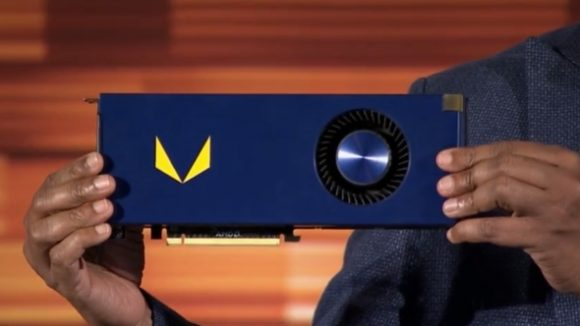
\includegraphics[height=45mm]{Figures/AMD_Radeon_Vega_Frontier_Edition.jpg}
\vspace{4cm}

% Title, author and degree
\vspace{1.0cm}
{\FontLb Taking GPU Beyond its Conventional DVFS Limits: Application to Deep Learning} \\ % <<<<< EDIT TITLE
%\vspace{0.2cm}
%{\FontMn Subtitle (optional)} \\
%\vspace{1.9cm}
\vspace{2.6cm}
{\FontMb Francisco Soares Mendes} \\ % <<<<< EDIT NAME
\vspace{3.0cm}
{\FontSn \coverThesis} \\
\vspace{0.3cm}
{\FontLb Electrical and Computer Engineering} \\ % <<<<< EDIT COURSE
\vspace{1.0cm}
{\FontSn %
\begin{tabular}{ll}
 \coverSupervisors: & Dr. Nuno Filipe Valentim Roma \\ % <<<<< EDIT NAME
                    & Dr. Pedro Filipe Zeferino Tomás    % <<<<< EDIT NAME
\end{tabular} } \\
\vspace{1.0cm}
%{\FontMb \coverExaminationCommittee} \\
\vspace{0.3cm}
%{\FontSn %
%\begin{tabular}{c}
%\coverChairperson:     Prof. Full Name          \\ % <<<<< EDIT NAME
%\coverSupervisor:      Prof. Full Name 1 (or 2) \\ % <<<<< EDIT NAME
%\coverMemberCommittee: Prof. Full Name 3           % <<<<< EDIT NAME
%\end{tabular} } \\
\vspace{1.5cm}
\vspace{2cm}
{\FontMb January 2020} \\ % <<<<< EDIT DATE (corresponds to date of oral examination)
%
\end{center} % file "Thesis_FrontCover.tex"
\cleardoublepage

% ----------------------------------------------------------------------
%  Table of contents, list of tables, list of figures and nomenclature
% ----------------------------------------------------------------------

% Table of contents
%
\tableofcontents
\cleardoublepage 

% Set arabic numbering (1,2,...) after preface
%
\setcounter{page}{1}
\pagenumbering{arabic}

% ----------------------------------------------------------------------
%  Chapters
% ----------------------------------------------------------------------

%%%%%%%%%%%%%%%%%%%%%%%%%%%%%%%%%%%%%%%%%%%%%%%%%%%%%%%%%%%%%%%%%%%%%%%%
%                                                                      %
%     File: Thesis_Introduction.tex                                    %
%     Tex Master: Thesis.tex                                           %
%                                                                      %
%     Author: Andre C. Marta                                           %
%     Last modified :  2 Jul 2015                                      %
%                                                                      %
%%%%%%%%%%%%%%%%%%%%%%%%%%%%%%%%%%%%%%%%%%%%%%%%%%%%%%%%%%%%%%%%%%%%%%%%

\chapter{Introduction}
\label{chapter:introduction}

With the advent of Big Data, a massive amount of information is constantly being collected and analyzed to extract value out of it. The way to obtain the value is through the use of machine learning (ML) algorithms, capable of analyzing huge data sets and uncover relations and extract meaning out of the raw information. These algorithms are being run in all kinds of devices, from supercomputers to our smartphones and a tonic exists across all kinds of modern devices, they are Heterogeneous Computing Systems composed of traditional Central Processing Units (CPUs) and Graphical Processing Units (GPUs). The use of GPUs, with their highly parallel architecture, is bringing significant gains in the performance to the systems and the possibility of increased capabilities of the algorithms being run. 

The addition of this new processing device to the computers also brought the drawback added power consumption. However, unlike CPUs, where it is already common to see advance power techniques that control the frequency and voltage applied to the processor accordingly to the workload, on GPUs the dynamic scaling  of its frequency and voltage (Dynamic voltage and frequency scaling - DVFS) is still mostly relying on external factors such as the temperature of the die and the power that the system is requiring to the power supply. The use of GPUs in such different types of applications, from video games and rendering to scientific simulations and machine learning applications, makes it hard for manufacturers to optimize the DVFS parameters to couple with the different workloads.

In the case of machine learning algorithms, big efforts are being done to enable them to be run with minimum energy consumption. From optimizing specific parts of the GPUs architecture to achieve higher performance to the scheduling of the different kernels being run to maximize the performance and minimize the Dark Silicon phenomenon \cite{esmaeilzadeh_dark_2011}. However, if one looks to the nature of machine learning algorithms, the train of it is based on iterative and convergence processes, where small imprecisions of the computation, still leads to correct outputs. These types of applications are called Imprecise Tolerant (IT) applications and their hidden property of tolerance against imprecision can be exploited to increase the efficiency of the circuits running them. In this case, two types of approaches can be made: the creation of custom computational blocks that natively have sources of control imprecision intending to reduce the power consumption \cite{mahdiani_efficient_2017} or, try to use regular GPUs outside of the circumscribed voltage and frequency margins defined by the GPU manufacturer. While the first approach will require the addition of more hardware to the devices and contribute to the Dark Silicon phenomenon, the second has the great benefit of allowing improvements of the current hardware in the market. 

To verify the feasibility of enabling a degree of imprecise computation in a regular GPU, a convolution neural network (a type of machine learning algorithm specialized for image processing) is trained to identify handwritten numbers of the MNIST data set. This neural network is trained on a heterogeneous computer equipped with an AMD GPU, first with the conventional DVFS parameters and then outside of it. It is verified that it is possible to under-voltage the GPU core 170mV from the default1150mV without any degradation on both the performance of the GPU (required time to train the model) and the achieved accuracy at the end of the training session. More importantly, this reduction on the supplied voltage led to a reduction of 40.48\% of the maximum required power,  28.81\% reduction on the average power and a 26.92\% reduction of the total required energy to train the model.

This result shows that there is space to be explored outside of the conventional DVFS parameters when Imprecise Tolerant applications are being executed.


%%%%%%%%%%%%%%%%%%%%%%%%%%%%%%%%%%%%%%%%%%%%%%%%%%%%%%%%%%%%%%%%%%%%%%%%
\section{Main Objectives}
\label{section:objectives}

The objective of this dissertation is to create a new DVFS mechanism that is aware of the nature of the application being run and the results that are being produced by it, to reduce the total power consumption of the GPU. With this new mechanism, it will be possible to enlarge the voltage and frequency margins, working outside of the conventional DVFS limits in current hardware. 

With this objective, it is first necessary to test different classes of machine learning algorithms, to find their imprecision tolerance and what are the impacts of running them with not default DFVS parameters. Parallel to it, a way of acquiring meaningful performance counters in runtime about the running application has to be found. With these two modules, it will be possible to validate how big is the impact of running applications in such a manner and understand how does the performance metrics relate to the voltage and frequency. The acquired relations will be used to create a model that tries to minimize energy consumption by controlling the voltage and frequency of the GPU. The last step of the presented work is to test the new DVFS aware model and understand the degree of improvement achieved. Figure \ref{fig:thesisObj} graphically shows the temporal relation between the different objectives to be performed during the dissertation.

\begin{figure}[!htb]
  \centering
  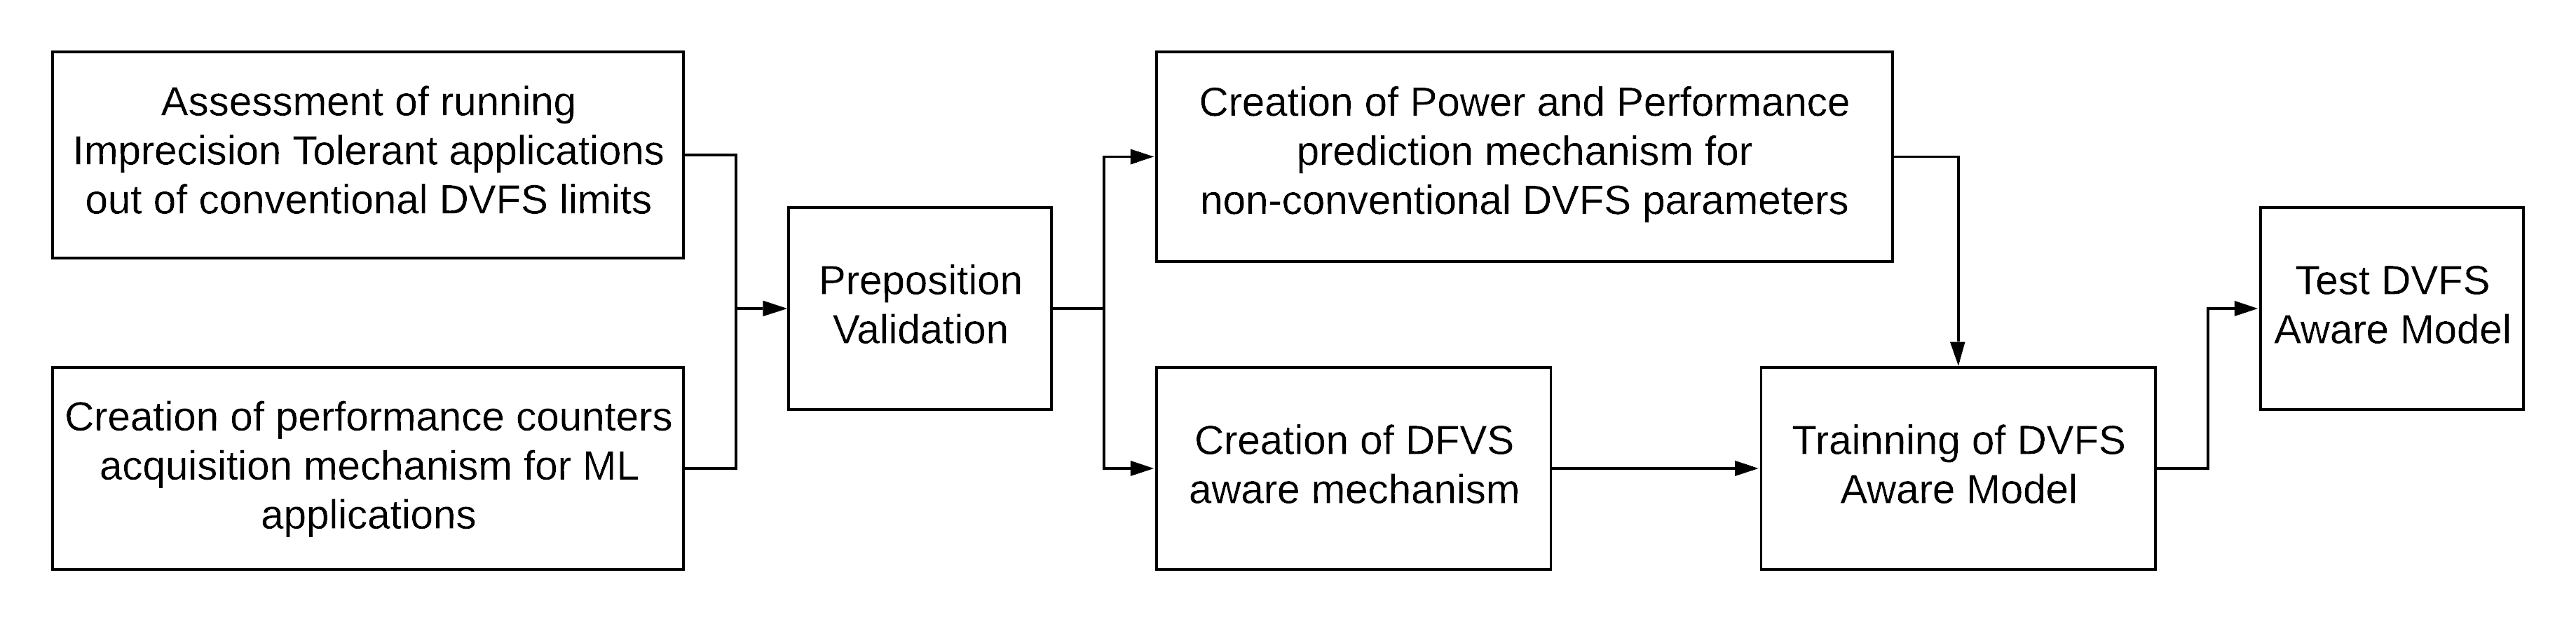
\includegraphics[width=1\textwidth]{Figures/Introduction/Dissertation_Objectives.png}
  \caption{Flowchart of dissertation objectives.}
  \label{fig:thesisObj}
\end{figure}

\section{Report Outline} % file "Thesis_Introduction.tex"
\cleardoublepage

%%%%%%%%%%%%%%%%%%%%%%%%%%%%%%%%%%%%%%%%%%%%%%%%%%%%%%%%%%%%%%%%%%%%%%%%
%                                                                      %
%     File: Thesis_Background.tex                                      %
%     Tex Master: Thesis.tex                                           %
%                                                                      %
%     Author: Andre C. Marta                                           %
%     Last modified :  2 Jul 2015                                      %
%                                                                      %
%%%%%%%%%%%%%%%%%%%%%%%%%%%%%%%%%%%%%%%%%%%%%%%%%%%%%%%%%%%%%%%%%%%%%%%%

\chapter{State of the Art}
\label{chapter:stateoftheart}


To reflect the recent GPUs use cases and the efforts being made in the pursuit of improving the performance and minimizing the energy consumption of them, this chapter provides an overview of the architecture of modern GPUs, with a brief specialization on the AMD GNC architecture. It also presents what kinds of power savings techniques are currently being employed in the existent hardware and a review of the literature related to the effects that the change of the frequency and voltage have on different workloads. The relevance of this works emerges from the lack of literature on the effects of undervolting the GPU, the objective of this dissertation. This is due to the lack of support for the control of this parameter on NVIDIA GPUs that is allowed by the novel AMD software stack used on this work. Furthermore, an overview of power and performance models is provided, highlighting the different techniques used to predict these two metrics. 


%%%%%%%%%%%%%%%%%%%%%%%%%%%%%%%%%%%%%%%%%%%%%%%%%%%%%%%%%%%%%%%%%%%%%%%%
\section{General Purpose Computing on GPUs}
\label{section:gpuarch}

A GPU is a highly parallel programmable processor, that is built to perform the same instruction on a set of data, belonging to the category of processors of \textit{Single Instruction Multiple Threads} - SIMT. When referring to GPUs, it is still common to be talking about their graphics capabilities, however, more and more programs are taking advantage of their highly parallel architecture to accelerate applications. The use of GPUs in general programming commonly referred to as GPGPU - General Purpose Graphical Processing Unit was first led by the development of CUDA \cite{noauthor_cuda_2017} by NVIDIA and OpenCL \cite{noauthor_opencl_2013} by Khronos Group. CUDA and OpenCL are both parallel computing platforms and application programming interface (API) that allows developers to create GPU-accelerated applications, where the computation can be divided between the CPU and GPU. However, the first versions of these frameworks treated the GPU as a slave device, providing a set of directives that allow the CPU (master device) to transfer data, synchronize and control the GPU.  Though, to take full advantage of the GPU architecture and create a true heterogeneous system, the CPU and GPU collaborate more efficiently. This lead, in 2012, the HSA Foundation to propose the Heterogeneous System Architecture HSA \cite{hwu_heterogeneous_2015} framework that acts as an intermediary low-level API to provide improved coordination and communication for heterogeneous computing systems.  More recently, AMD introduced the Radeon Open Computing platform (ROC) \cite{noauthor_radeonopencompute/rocm_2019}. ROC, like CUDA and OpenCL, provides a set of tools that allow developers to create heterogeneous applications. The added benefits of ROC are that it is built on top of the HSA runtime API and that exposes the framework in a wider set of programming frameworks like OpenCL, HC++, and HIP.

The development of improved frameworks and programming methodologies are making GPUs the prime tool to accelerate big-data applications and deep learning algorithms. GPUs can outperform CPUs in both throughput and energy efficiency. In this section, it will be provided a general overview of the GPU architecture, followed by an exploration of architectural techniques that are being employed to reduce power consumption and increase the efficiency of these devices.


\subsection{General Overview of GPU Architecture}
The architecture of the GPU can be roughly divided into computation and memory components. The computation part is composed of the vertex shader, the rendering engine, and the RISC processors. The vertex shader and rendering engine are inserted on the graphics pipeline and are not generally used on GPGPU applications. The RISC processors are responsible for the GPU programmable calculations, and depending on the manufacturer, can be called streaming multiprocessors (SMs) in NVIDIA GPUs \cite{nvidia_cuda_nodate} or computing units (CU) in AMD GPUs \cite{amd_amd_nodate}. To support thousands of concurrent threads simultaneously, each CU is made up of hundreds of execution units. Every CU has a statically allocated register file, where each thread can reserve a physical part of it \cite{jing_energy-efficient_2013}. To enable concurrent execution of multiple threads in a single CU and allow low-overhead context switch, modern GPUs provide a large register file, where the context of all active threads can be stored. For reference, in the AMD GNC architecture, each CU has 49152 (32-bit) registers.

In terms of memory, both the AMD and the NVIDIA GPU present a 3 level hierarchy system: a global memory, accessible by all processors units (generally referred as video memory); a shared memory associated with each SM or CU, accessible by the processing units of that SM or CU; and a set of read-only caches for constants and textures.

A GPU from AMD will be used to conduct the experimental part of this dissertation. For that reason, a more in-depth analysis of the architecture and framework from this manufacturer will be provided and the terminology used by it will be adopted. However, the presented work is independent of the hardware and terminology itself.

\subsection{AMD Graphics Core Next}

The AMD Graphics Core Next (GCN) \cite{amd_radeons_nodate}  architecture includes both the GPU microarchitecture as well as the instruction set of the processor unit. The architecture was first released in 2012, and it is already in its fifth iteration with the codename Vega. The Vega microarchitecture is based on a multiprocessor chip with an array of 64 RISC SIMT processors called Compute Engine (CE). Respectively, each CE is constituted by 64 Next Compute Units (NCU), performing a total of 4096 stream processors, also called Compute Units. The interface between the GPU and the Host is done throw the Peripheral Compute Interconnect Express (PCIe). Figure \ref{fig:Vega10arch} represents the logical organization of a Vega GPU.  

\begin{figure}[!htb]
  \begin{subfigmatrix}{2}
    \subfigure[Chip block diagram, example with 4 CEs]{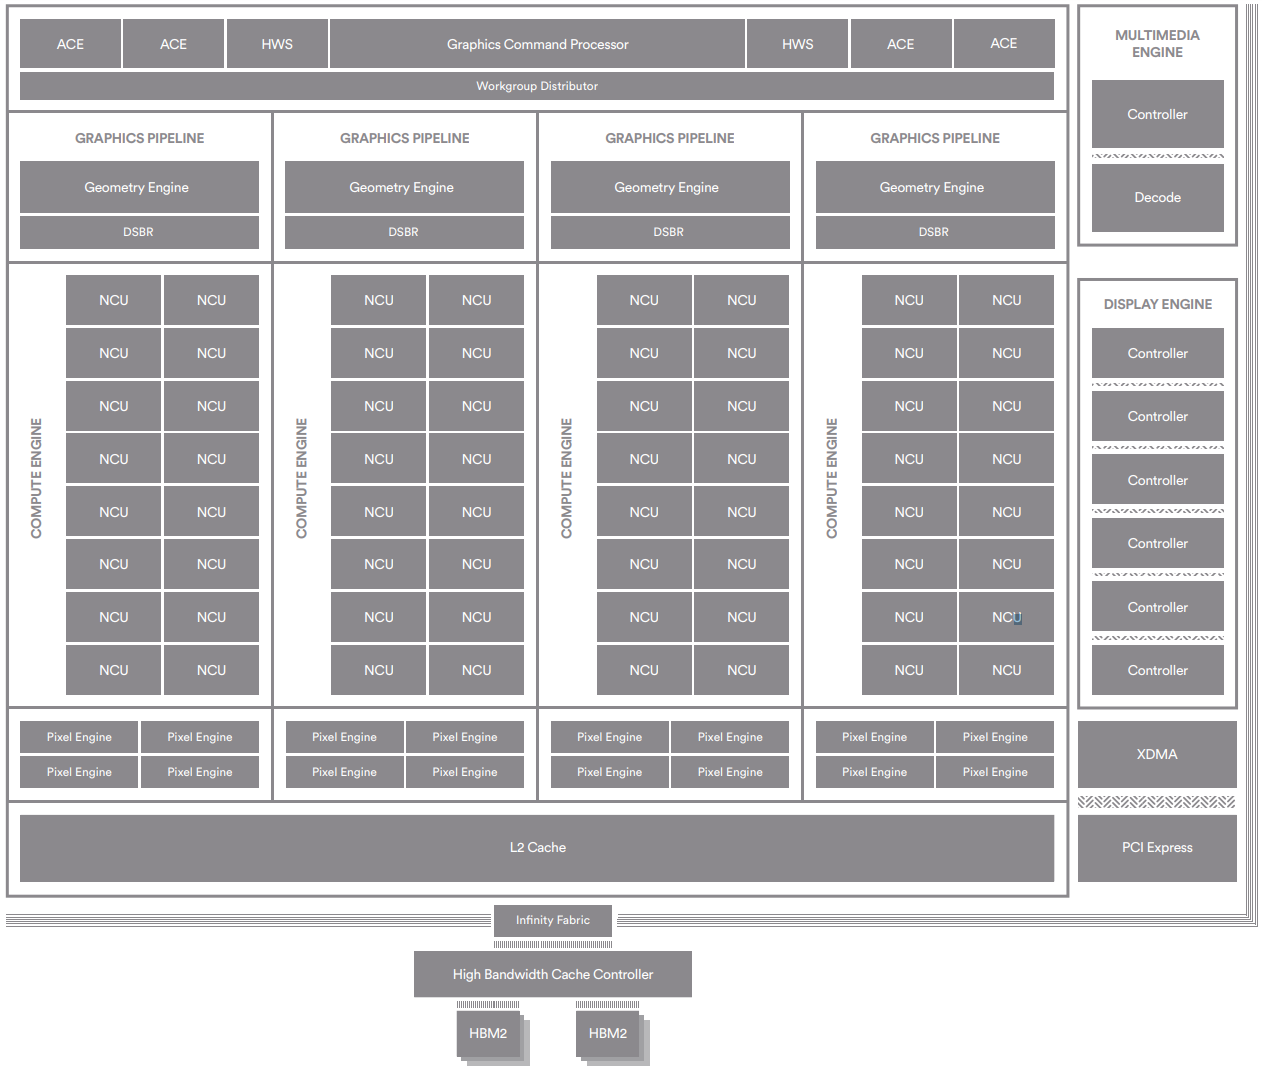
\includegraphics[width=0.7\linewidth]{Figures/StateArt/Vega10_microarchitecture.png}}
    \subfigure[NCU]{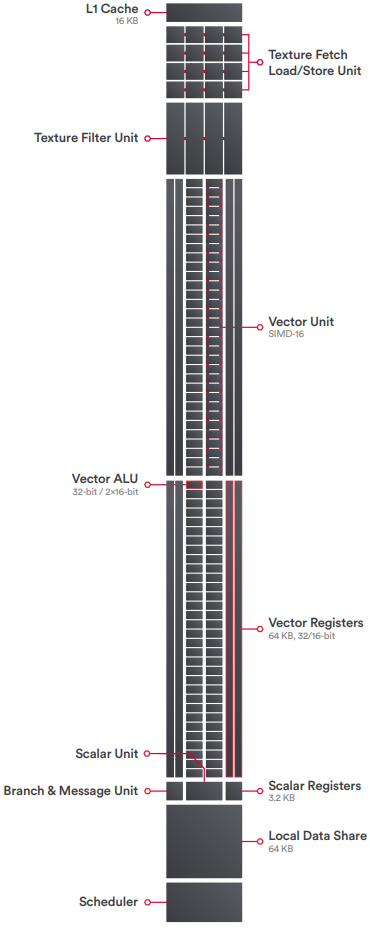
\includegraphics[width=0.29\linewidth]{Figures/StateArt/NCU.png}}
  \end{subfigmatrix}
  \caption{AMD's Graphics Core NExt logical Organization.}
  \label{fig:Vega10arch}
\end{figure}

In the fifth iteration of the GNC microarchitecture, AMD introduced a new memory hierarchy and support for High-Band Memory 2 (HBM2). In a conventional memory arrangement, the registers of each processing element pull data from a set of L1 caches, that, in turn, access the global L2 cache. Finally, the L2 cache system provides access to the GPU's video memory. This arrangement implies that the video memory has the entire working set of data and resources in order to provide high-bandwidth and low-latency access to data. However, in complex graphical scenes or while working GPGPU applications with large datasets, the total video memory may not be big enough to store all the data. In the Vega microarchitecture, by utilizing a  High-Bandwidth Cache Controller (HBCC), AMD made it possible to utilize the local video memory like a last-level cache. In this arrangement, when a missing piece of data, not currently stored in the local memory, is needed by the CUs, the GPU can pull just the necessary page memory from the host. In this setup, instead of the GPU stalling, while the entire missing resource is copied from the host throw the PCIe bus, it just needs to wait for the smaller page memory to be transferred, resulting in significantly decreased memory access times. The GPGPU applications take great advantage of this memory hierarchy since it enables the use of bigger datasets than the ones that could fit in video memory.

In the development of the work of this dissertation, a Radeon Vega Frontier Edition GPU is used. Table \ref{tab:gpusepcs} summarizes the most important specifications of the architecture of this device.

\begin{table}[!htb]
    \renewcommand{\arraystretch}{1.2} % more space between rows
    \centering
        \begin{tabular}{lc}
            \multicolumn{1}{c}{\textbf{}} & \multicolumn{1}{l}{\textbf{Radeon™ Vega Frontier Edition}} \\ \hline
            Base Architecture             & Vega GNC                                                   \\
            \#Compute Units               & 64                                                         \\
            \#Stream Processors           & 4096                                                       \\
            GPU Memory Size               & 16 GB                                                      \\
            Thermal Design Power          & 300 W                                                      \\ \hline
        \end{tabular}
    \caption{Characteristics of the used GPU device}
    \label{tab:gpusepcs}
\end{table}

\subsection{Radeon Open Compute platform}

The Radeon Open Compute (ROC) \cite{noauthor_radeonopencompute/rocm_2019} platform provides support for a set of frameworks and tools to allow developers to program and control the AMD GPUs. Figure \ref{fig:rocmplatform} shows the high-level organization of the platform. The platform includes a set of tools that allows developers to access ROC Kernel Driver data. In the following subsections, two of those tools, the ROCM-SMI \cite{noauthor_radeonopencompute/roc-smi_2019} and ROC-Profiler \cite{noauthor_rocm-developer-tools/rocprofiler_2019} tools, used on the development of this work, are described.

\begin{figure}[!htb]
  \centering
  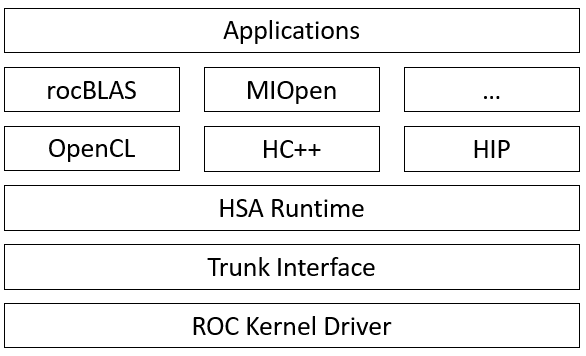
\includegraphics[width=0.5\textwidth]{Figures/StateArt/rocStack.png}
  \caption{Organization of the ROC platform.}
  \label{fig:rocmplatform}
\end{figure}

\subsubsection{ROCM-SMI}
The ROCm System Management Interface (ROC-SMI) \cite{noauthor_radeonopencompute/roc-smi_2019} is a user-friendly command-line application for manipulating the Radeon Open Compute Kernel (ROCK),  using it, is possible to know and control the state of the GPU device. The application uses sysfs files to query and manipulate the device kernel using the libsensors library \cite{noauthor_libsensors3:_nodate}.

From the set of query and control directives enabled by ROC-SMI, the following are of particular interest for the topic of this dissertation:

\begin{itemize}
\item \textbf{GPU utilization:} Retrieves the current utilization rates for the device's major subsystems, one value for the processing core and other for the main device memory. The rate is computed over a specific time interval set on the libsensors library. The processing core utilization reflects the percentage of time that the GPU core was being utilized to perform computations. In contrast, the main device memory utilization reflects the times on which the memory was being read or written.

\item \textbf{GPU power}: Retrieves the average power used by the device. Similarly to the utilization rate, the average power computed over the same time interval, during which a defined number of power samples are taken.

\item \textbf{Clock rate and voltage level:} Retrieves both the currently applied clock frequency and voltage level to the GPU core and the main device memory. It also displays two tables, the first, showing the eight pairs of clock frequency/voltage level of the GPU core and the second, showing four pairs of the same parameters related to the device memory. These two tables, correspondent to the 8 and 4 performance levels that the device kernel can apply to the GPU core and memory correspondingly.
\end{itemize}

The ROC-SMI interface also allows querying the device temperature, the current fan speed, and the selected performance level.

ROC-SMI also provides a mechanism to control and change device parameters such as:
\begin{itemize}
\item \textbf{Set clock rate and voltage level:} Set the clock frequency and the voltage level of any of the performance levels of both the GPU core and memory. 
\item \textbf{Set performance level:} Allows the user to select the desired performance level of the GPU core and device memory, disabling the driver automatic performance level management system.
\item \textbf{Reset clock rate and voltage level:} Resets the clock rates and voltage level to the default values.
\end{itemize}

Additionally, the interface allows the user to manually set the fan speed, necessary to guarantee the same temperature level for all executed tests

The versatility and total and independent control of the clock rate and voltage level of the device allowed by ROCM-SMI and the libsensors library was the defining factor for choosing an AMD GPU over the more popular options of NVIDIA. In the development of the work presented in this dissertation, an exploration of the voltage level is undertaken, and only the AMD platform allows for independent control over this variable.

\subsubsection{ROC-Profiler}

The Radeon Open Compute Profiler \cite{noauthor_rocm-developer-tools/rocprofiler_2019} is a profiling and tracing library for applications developed using any of the programming frameworks available on the ROC platform (OpenCL, HC++, HIP) \cite{sun_evaluating_2018}. The library gives access to the performance counters of AMD GPUs, allowing developers to configure the start, stop, read and reset of the physical registers on the microarchitecture that count the number of events (number of instructions per type, cache hits/miss) that the device is performing.

The instrumentation of applications with the API calls to ROC-Profiler allows for close monitoring of the type of operations being performed. The use of this tool can give valuable insights about the relation that the running code has with the utilized frequency and voltage and the produced result.


%%%%%%%%%%%%%%%%%%%%%%%%%%%%%%%%%%%%%%%%%%%%%%%%%%%%%%%%%%%%%%%%%%%%%%%%


\section{Dynamic Voltage and Frequency Scaling}
\label{section:dcvf}

The widespread use of GPUs in both supercomputers as on personal machines comes at the cost of a significant increase in the power consumption of the complete system. Whereas a typical modern CPU consumes about 50 to 100W, it is common to see GPUs rounding that value to 200 to 300W of power. With these figures, it is indispensable the use of energy efficiency techniques to try to reduce power consumption.

On any CMOS circuit, the total power consumed is decomposed into the dynamic and static parts. The dynamic power relates to the act of the transistors flipping their stages, and correspond to the power of charging and discharging the internal net capacitances. This value is proportional to the frequency that this change occurs. Equation \ref{eq:dynpower} represents the general form for dynamic power, where \textit{a} represents the utilization factor, \textit{C} the total capacitance of the circuit, \textit{V} the transistors supplied voltage and \textit{f} the operating frequency \cite{gonzalez_supply_1997}.

\begin{equation}
    P_{dynamic} = aCV^2f
    \label{eq:dynpower}
\end{equation}


On their turn, the static part of the power consumption is generated by $P_{leakage}$, $P_{short-circuit}$ and $P_{DC}$ \cite{mei_survey_2016}. The leakage power is independent of the transistors flip, and it represents the flow of electrons between the transistors' source, drain, and gate, known as current leakage. The short-circuit power comes from the instantaneous short-circuit connection between the supply voltage and the ground when the transistor flips. Finally, the Direct Current (DC) power corresponds to the power needed for powering the circuit. Equation \ref{eq:cmospower} represents the total power consumption sources.

\begin{equation}
    P_{total} = P_{dynamic} + P_{leakage} + P_{short-circuit} + P_{DC}
    \label{eq:cmospower}
\end{equation}

The dynamic power dominates the total power consumption of a circuit, however, with the reduction of the manufacturing size of the transistor seen nowadays, the static power is also contributing heavily \cite{s._hong_modeling_2012} \cite{hong_integrated_2010}. As a common reference, due to the higher height of the dynamic power on the total power consumption, the power used by a circuit changes linearly with the clock frequency and quadratically with the supplied voltage.


By intelligently controlling the clock frequency, the necessary voltage for stable operation of the circuit can also be reduced, leading to power savings. However, the reduction of the operating frequency harms the pic performance of the circuit, so a careful scaling of voltage/frequency needs to be done in run-time. The "on the fly" control of these parameters is called Dynamic Voltage and Frequency Scaling (DVFS). This power management technique allows for an energy efficiency improvement by matching the GPU utilization to the voltage and frequency apply to it.

In general, modern GPU boards have independent control over two pairs of frequency and voltage. Each pair or domain acts on a distinct part of the GPU, intending to maximize the performance or reduce the power consumption. The first domain concerns the GPU core, acting on all CUs, the cache, and the interconnection fabric. The second affects the DRAM chips that compose the video memory. 

The clock frequency is an independent control variable, and its change is reflected directly on the performed achieved by the GPU. An increase in the clock frequency of the core results in an improvement of the CU execution speed, while the same change in the memory frequency will increase the DRAM I/O throughput \cite{mei_survey_2016}. The voltage level of each domain is dependent on the clock frequency and is computed based on tests performed by the manufacturer that ensure the correct operation of the circuit, independently of the workload.

Both AMD and NVIDIA have on their products the concept of performance levels, that is, a set of pairs of frequency and voltage that can be applied to the many components of the GPU. These vary from low power and performance levels to high performance and high power ones. The idea of having multiple performance levels is to be able to always be at the best point of operation.  In the case of AMD, the GPU core has eight possible pairs, table \ref{tab:gpucorelevels} shows the reference values of frequency and voltage for each of the core performance levels, while the GPU memory has only four, table \ref{tab:gpumemlevels}. Through the use of software like ROC-SMI \cite{noauthor_radeonopencompute/roc-smi_2019} the user can input the desired combination of values for each level, allowing for an almost continuously selection of values for the frequency and voltage within the specifications range. For example, on the Vega 10 Frontier Edition used on the experimental work of this thesis, the GPU core frequency can be set between 852 and 1980 MHz and the GPU memory frequency between 167 and 1500 MHz. In turn, the voltage can be set between the 800 and 1250 mV. As stated before, the primary benefit of AMD over NVIDIA's solution is that this manufacturer allows for the override of the automatic computation of the GPU voltage. This difference is of significant importance since it allows finer control of the DVFS values and a more interesting possibility of exploration of the voltage level.

\begin{table}[!htb]
\renewcommand{\arraystretch}{1.2} % more space between rows
\centering
\begin{tabular}{ccc}
\textbf{Level} & \textbf{Frequency {[}MHz{]}} & \textbf{Voltage {[}mV{]}} \\ \hline
0              & 852                          & 800                       \\
1              & 991                          & 900                       \\
2              & 1138                         & 950                       \\
3              & 1269                         & 1000                      \\
4              & 1348                         & 1050                      \\
5              & 1440                         & 1100                      \\
6              & 1528                         & 1150                      \\
7              & 1600                         & 1200                      \\ \hline
\end{tabular}
\caption{GPU Core Levels of Frequency and Voltage of AMD Vega 10 Frontier Edition}
\label{tab:gpucorelevels}
\end{table}

\begin{table}[!htb]
\renewcommand{\arraystretch}{1.2} % more space between rows
\centering
\begin{tabular}{ccc}
\textbf{Level} & \textbf{Frequency {[}MHz{]}} & \textbf{Voltage {[}mV{]}} \\ \hline
0              & 167                          & 800                       \\
1              & 500                          & 900                       \\
2              & 800                          & 950                       \\
3              & 945                          & 1000                      \\ \hline
\end{tabular}
\caption{GPU Memory Levels of Frequency and Voltage of AMD Vega 10 Frontier Edition}
\label{tab:gpumemlevels}
\end{table}

\subsection{Control Mechanism}

The correct choice of the most appropriate performance level for each of the GPU clock domains is one of the topics of more research from both the manufactures and researchers. The correct design of the DVFS controller has a significant impact on the energy efficiency of the GPU.

The first implementations of GPU DVFS controllers took direct inspiration from the CPU DVFS and can be largely classified into interval-based, inter-task, and intra-task DVFS algorithms \cite{boyer_improving_2013}. 

\subsubsection{Interval-based}

Interval-based algorithms rely on the periodical measurement of the utilization of the device, setting the next frequency and voltage based on the average measurement of utilization. The utilization $U_{i}$ reflects the percentage of working time, $w_{i}$, spent by the GPU over the last time frame  $Tf_{i}$ and can be formulated following equation \ref{eq:utilization}.

\begin{equation}
    U_i=\frac{w_i}{Tf_i}
    \label{eq:utilization}
\end{equation}

By applying arithmetic, geometric, or weighted average, or a more complex algorithm, over the last \textit{n} \textit{U} measurements,  the next utilization, $U_{i+1}$ is predicted. If the predicted value surpasses pre-determined upper and lower thresholds, the frequency is adjusted up or down accordingly \cite{seongki_gpgpu-perf:_nodate}. 
A \textit{governer} is a set of parameters such as frequency and voltage tables, thresholds and utilization prediction algorithm that controls how the interval-based DVFS works, by choosing a different \textit{governer}, the DVFS system can react differently to the same workload. Figure \ref{fig:DVFSprocedure} schematizes the periodic procedure executed by the DVFS system \cite{seongki_gpgpu-perf:_nodate}. 

\begin{figure}[!htb]
  \centering
  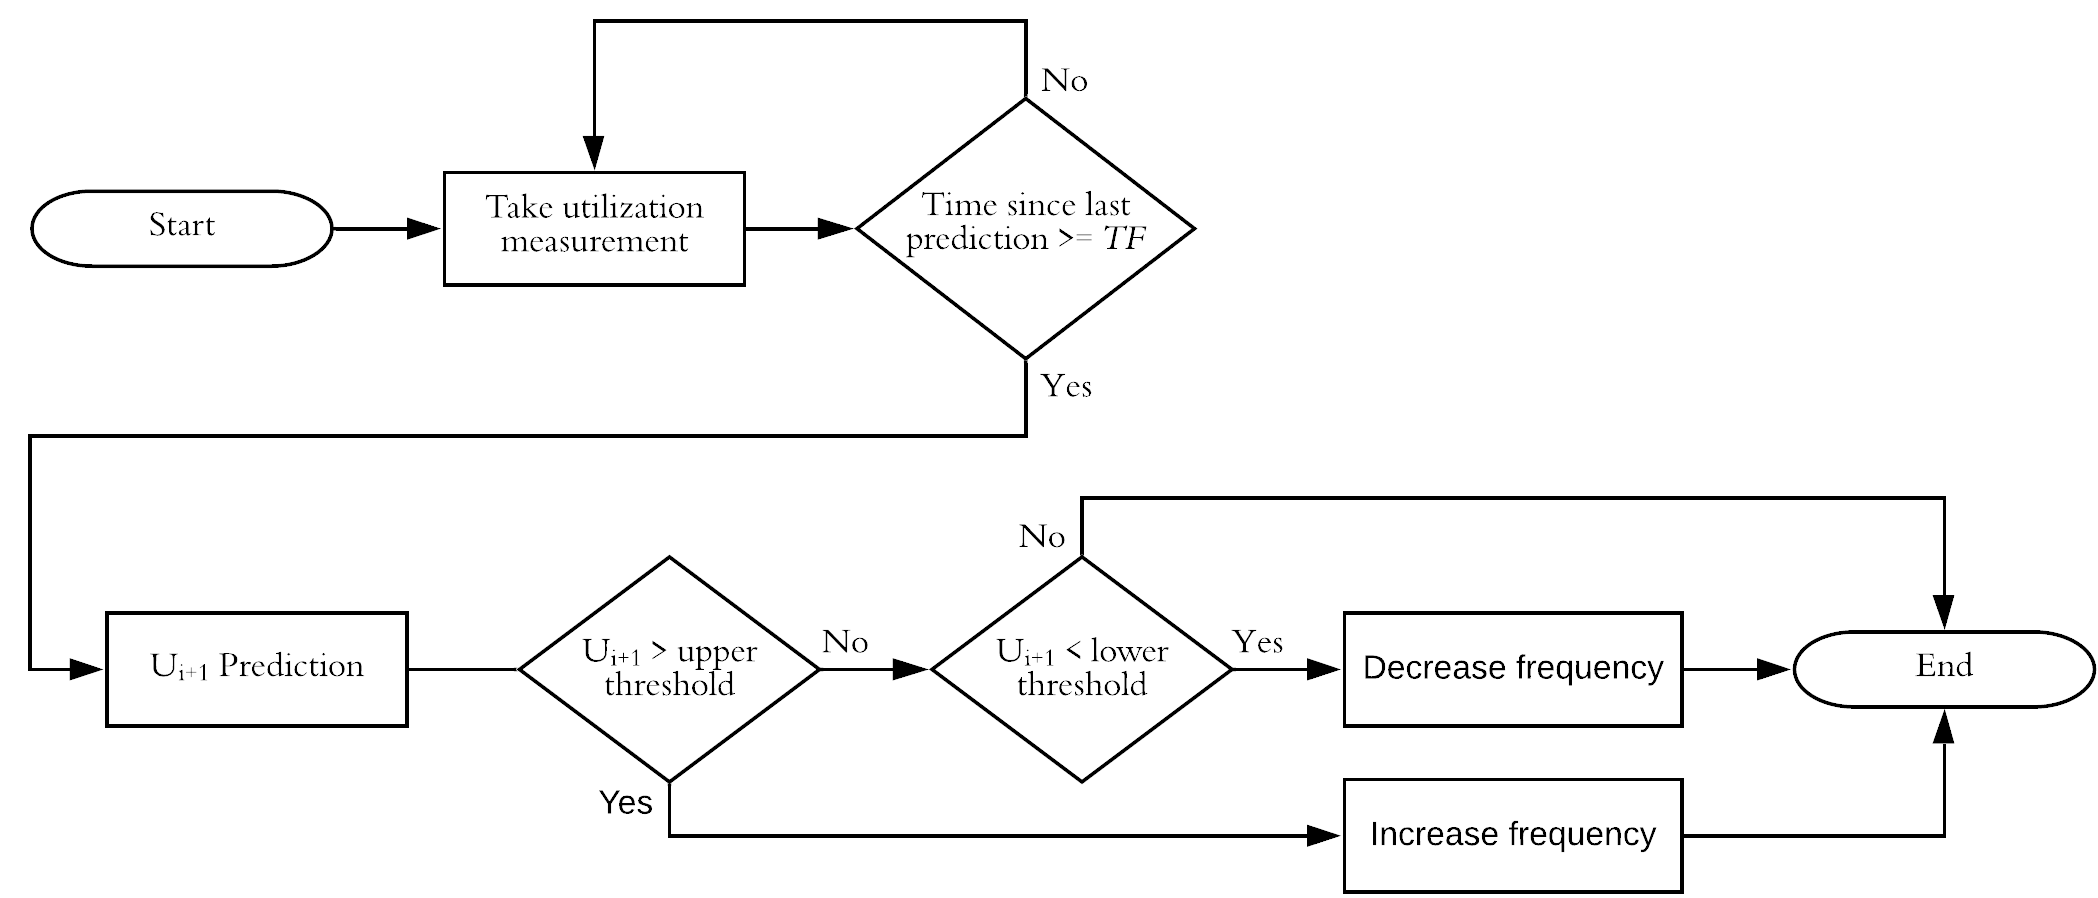
\includegraphics[width=0.5\textwidth]{Figures/StateArt/DVFSprogram.png}
  \caption[Controller]{DVFS procedure.}
  \label{fig:DVFSprocedure}
\end{figure}

\subsubsection{Task-based}

Task-based DVFS algorithms analyze the source code and the task profiling results (performance counters values) to determine the optimal frequency/voltage. This type of algorithm is composed of an intra-task and an inter-task analysis \cite{noauthor_time_nodate}. The intra-task part decomposes the execution of the task or a process into the on-chip computation and off-chip access latencies and. Based on the results,  the optimal GPU core and memory frequency are determined accordingly to the ratio between the two types of execution. Inter-task mechanisms utilize the intra-task results, assigning a signature to each type of task/process. By analyzing, in run-time, the performance counters, and using a lookup table that stores the signatures, the optimal frequency/voltage is set for the sequence of tasks being executed.

In general, the challenges of creating a better GPU DVFS relates to three factors. The GPU power management is very limited, the lack of accurate quantitative GPU DVFS performance and power estimation tools, and the fact that the GPU architecture design is still evolving rapidly, which makes the strategies applied to one architecture design have different outcomes on the next iteration of it \cite{mei_survey_2016}. The observed results show that strategies like scaling up the processor frequency, race-to-idle  \cite{hoffmann_racing_2013} or "racing" \cite{kim_racing_2015}, when a task is launched in the pursuit of finishing it as fast as possible and return to an idle state prof to increase the energy efficiency of CPUs, however, that assumption not always results in the same outcome for GPUs \cite{kim_racing_2015}. 

\subsubsection{AMD DVFS Mechanism Example}

The control mechanism of the GPU DVFS used nowadays by both AMD and NVIDIA, schematized on figure \ref{fig:DVFSmechanism}, is primarily an interval based one. The most recent AMD GPU DVFS mechanism is called Adaptive Frequency and Voltage Scaling (AVFS) \cite{amd_polaris_nodate}. AFVS takes into account the voltage levels across the different parts of the GPU, the die temperature, the frequency and, the total power consumption. The objective of the controller is to maintain the total power consumption within the required power and temperature envelope, this is, for a given power target, when launching a new task, the GPU tries to achieve the highest possible frequency (highest performance level). For that, it adjusts the voltage level to the one required to correct functioning. With the use of the highest performance level, power, and temperature increases, when one of these parameters achieves the limit, the GPU decreases to a lower performance level to maintain itself within the power and temperature target. 

\begin{figure}[!htb]
  \centering
  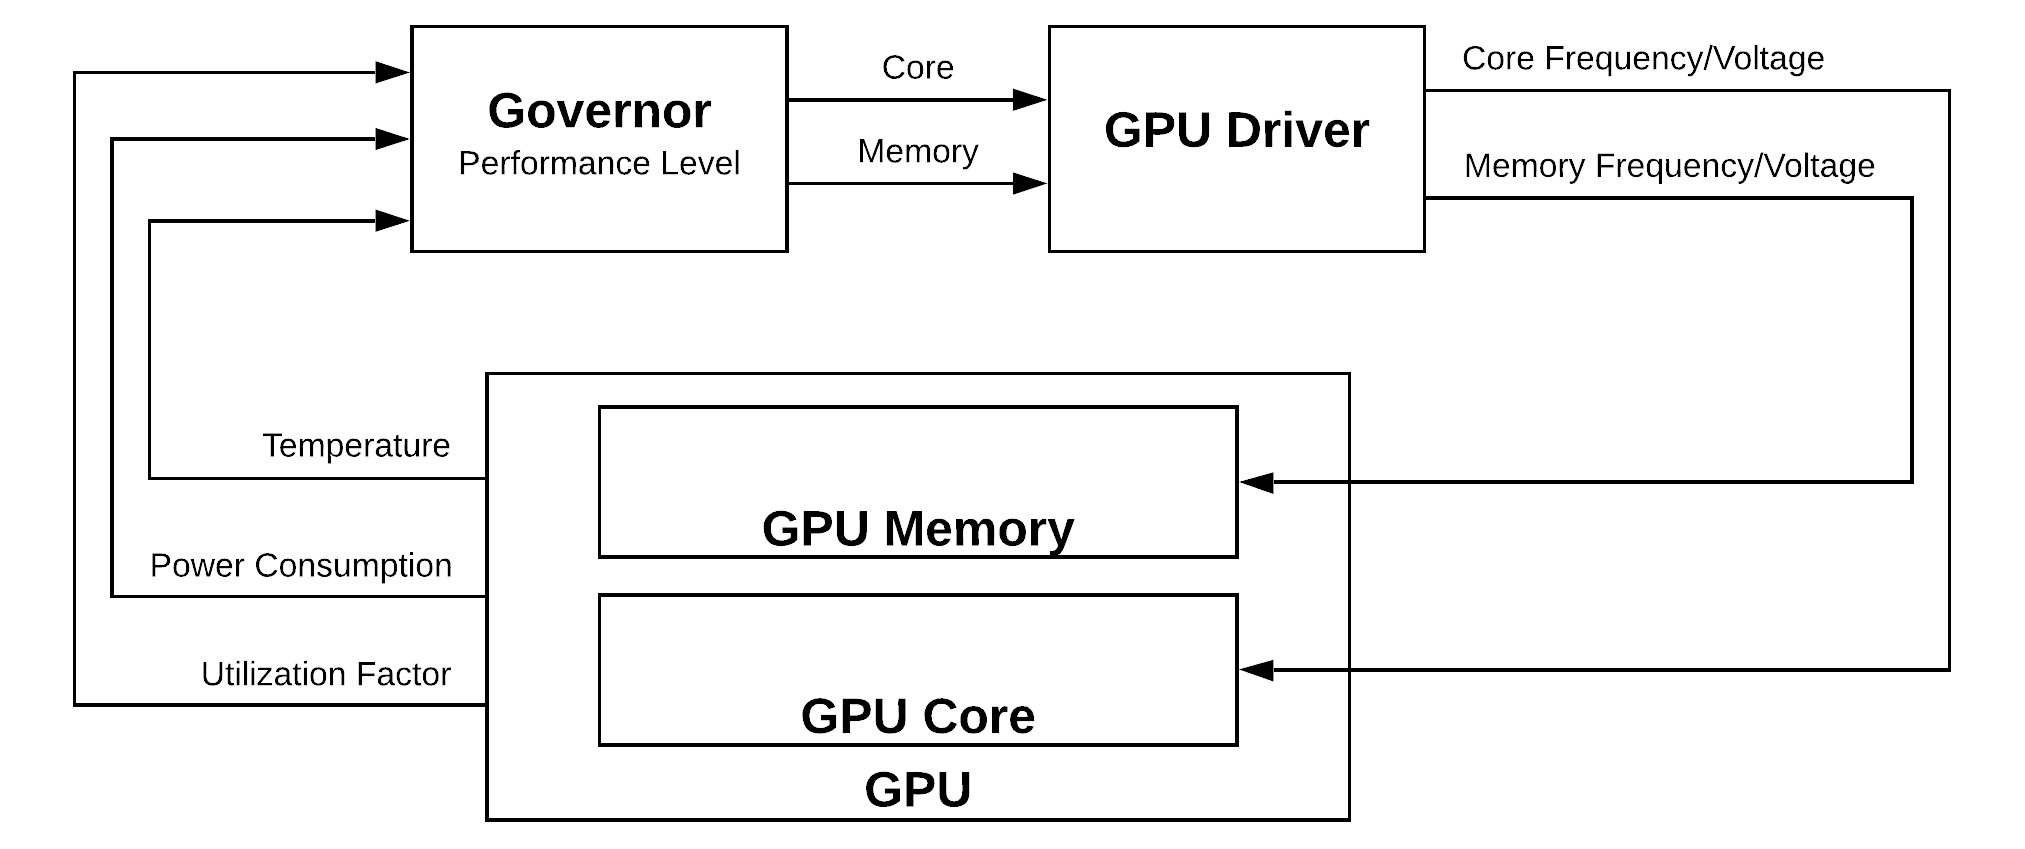
\includegraphics[width=0.75\textwidth]{Figures/StateArt/DVFS.png}
  \caption[Controller]{DVFS control mechanism.}
  \label{fig:DVFSmechanism}
\end{figure}

The major drawback of the current implementation of GPU DVFS is not taking into account the type of task that the GPU is solving. The dominant control mechanism still considers the GPU as a block box and controls its DVFS settings, only looking to outside parameters. The black box approach is enabling significant improvements in the energy efficiency of the device; however, it lacks the optimization of the frequency/voltage to the type of workload. For instance, a given application can be compute-bound or memory-bound, depending on if the time that it takes to performed is limited by the processor performance or the memory bandwidth and latency. This binary classification of applications also depends on the frequency of the core and memory. The same application can be compute-bounded at a low core frequency, but be memory-bounded at an higher core frequency \cite{guerreiro_dvfs-aware_2019} (the bottleneck switches from the processing elements to the memory). In the case of compute-bounded application, the limitation can be imposed by different components of the processor architecture, depending on the type of data (integer or floats) and the intended precision (size of the operands). If one compares the computation with the same type of operands but with different precision, for instance, 16 vs. 32 bits, even though the GPU is using the same arithmetic unit, the critical path for 32 bits operands is of increased length. That is, the maximum delay between the input and output for operations increases with the precision of the operands. Though, since the same clock frequency is used in both cases, the voltage level needs to be set at a level that ensures that the transistors flip at fast enough rate for the case with the highest precision. Considering that the manufacturers do not tune their devices to the minimum voltage level, to accommodate for manufacturing imprecisions and to leave a safe guard-band, the operating voltage of the circuits can be significantly reduced, leading to significant power savings. 

Overall, the minimum operating voltage of each performance level is set at a level high enough, that ensures the correct functioning of the processor, independently of the computations being performed. Nevertheless, it is possible to fine-tune the voltage and frequency if the type of task being executed is known.

\subsection{GPU DVFS Characterization and Effects}

Being the GPU such a widely used computation platform, in order to improve their performance and energy efficiency, it is of significant matter the characterization and analysis of the DVFS effects, mainly on understanding the impact of the different parameters on different workloads scenarios. A complete GPU DVFS characterization is explored in the literature using two methodologies. The first is experimental studies, where researchers use real GPUs to perform voltage and frequency scaling. Due to past dominance of NVIDIA over AMD \cite{noauthor_jon_nodate} \cite{mujtaba_amd_2019} and the fact that this manufacturer only offers limited support for independent voltage scaling tools, the majority of the work act solely on frequency scaling. The second approach uses simulators, like GPGPU-Sim \cite{noauthor_gpgpu-sim/gpgpu-sim_distribution_2019} and GPUWattch \cite{noauthor_gpu_nodate} \cite{leng_gpuwattch:_2013},  to simulate various scaling approaches like GPU core number scaling and per-core DVFS \cite{mei_survey_2016}. The benefit of using simulators over real hardware comes on the increased flexibility allowed by the previous, permitting for the experimentation of scenarios not supported by the frequency/voltage scaling tools provided by the manufacturers. In both methodologies, the studies act on the impact on performance and energy consumption/efficiency.

\subsubsection{Experimental}

Jiao \textit{et al.} \cite{jiao_power_2010} scaled the GPU core and memory frequency of an NVIDIA Tesla GTX 280 using three types of workload. First, a compute-bounded dense matrix multiplication application, second, a memory bounded application that performs dense matrix transpose and third, a mixed workload, Fast Fourier Transform (FFT) computation. The experimental study showed that for the same core-memory frequency settings, the three applications showed different performance and energy efficiency curves. While a computed bounded application showed to be insensitive to memory scaling, the mixed workload FFT takes advantage of high memory frequency and low core frequency. At last, the memory bounded application profits from both high core and memory frequency. In general, it was shown that energy efficiency could be determined by the instructions per cycle (IPC) and by the global ratio of memory transactions by computation transactions.

Ge \textit{et al.} \cite{ge_effects_2013} explored dense matrix multiplication kernel execution in more detail using an NVIDIA Kepler K20c GPU.  The work revealed that for this type of kernel (compute-bounded), the power used by the GPU and the achievable performance is linear to the GPU core frequency and that the total energy consumption had no relation to frequency scaling. In all the application tests used, the energy efficiency has a linear relation with the GPU frequency, with the highest energy efficiency achieved when the highest clock frequency was employed.

Abe \textit{et al.} \cite{abe_power_2012} introduced a global scaling procedure that combines the GPU core and memory frequency with the CPU frequency in order to minimize energy consumption. In the first experimentation, it was tried to optimize the computation of dense matrix multiplication with differing matrix sizes. Using this global scheme on a small matrix leads to a 28\% energy saving while using low GPU memory frequency and high GPU core frequency. The same procedure was then enlarged to a more diverse set of 33 benchmarks where all the possible combinations of a low, medium, and high GPU core and memory frequency were tested to find the optimal working settings. It was found that energy consumption can be reduced as much as 75\% within a performance loss of 30\% when the best settings were used. 

Mei \textit{et al.} \cite{mei_measurement_2013} conducted a more general experimentation using 37 GPU benchmarks. In this work, it was possible to observe that the effect of GPU DVFS depends on application characteristics. In all situations, the fine-tuning of DVFS per application (finding the lowest voltage level for the desired running frequency) always conveyed to an energy-saving of 20\%, on average, with only a 4\% performance loss. More recently, Mei  \textit{et al.}, expanded the previous work to analyze the relation between energy consumption and dynamic frequency scaling settings \cite{mei_survey_2016}. For the  Rodinia benchmark \cite{che_rodinia:_2009} it was found that some benchmarks increase the energy consumption linearly with frequency scaling while others are insensitive to the change of this parameter. In the particular case of GPU memory frequency scaling, the work revealed that underclocking this component can result in a 30\% energy decrease if the running application is not memory bounded. For the case of applications that the performance depends on the memory, decreasing the frequency, can lead up to 54\% energy increased due to the increased execution time. In this set of applications, overclocking the memory results in diminishing execution time with reduced overall energy consumption (in this case, the reduced computation time overshadows the memory energy consumption increase). Overall the relation between the DVFS settings and the energy consumption depends heavily on the application type, and a simple linear model (normally used by the GPU manufacturers) for DVFS settings is inadequate to achieve the best performance or energy consumption/efficiency.


%%%%%%%% EXPERIMENTAL

%ASurveyandMeasurementStudyofGPUDVFSonEnergyConservation
%Jiao et al. scaled the core frequency and the memory frequency of a NVIDIA Tesla GTX280 GPU with three typical applications: the compute-intensive dense matrix multiply, the memory - intensive dense matrix transpose, and the hybrid fast Fourier transform (FFT) [31]. The three applications showed different performance and energy efficiency curves with the same core-memory frequency settings: the dense matrix multiply was insensitive to memory frequency scaling, FFT benefited from low core frequency and high memory frequency, while dense matrix transpose needed both high core and memory frequency. They also found that the energy efficiency was largely determined by the instructions per cycle (IPC) and the ratio of the amount of global memory transactions over the amount of computation transactions. 
%Ge et al. applied fine-grained GPU core frequency and coarse-grained GPU memory frequency on a Kepler K20c GPU, and compared its effect to the CPU frequency scaling [19]. They found that for dense matrix multiply, both the GPU power and the GPU performance were linear to the GPU core frequency, and the GPU energy consumption was insensitive to frequency scaling. For their three tested applications, the highest GPU frequency always resulted in best energy efficiency, differing from the CPU DVFS. 
%In our previous work, we scaled the core voltage, the core frequency and the memory frequency of the Fermi GTX560Ti GPU, with a set of 37 GPU applications [47]. We found that the effect of GPU DVFS depends on the application characteristics. The optimal setting to consume the least energy was a combination of appropriate GPU memory frequency and core voltage/frequency. We observed an average of 20% reduction of energy consumption with only 4% of performance loss. 
%Abe et al. combined the GPU core frequency, the GPU memory frequency and the CPU core frequency scaling together, on the NVIDIA Fermi GTX480 GPU [3]. They performed the frequency scaling with dense matrix multiply of various matrix sizes. They could save as much as 28% of the system energy with a small matrix size, low GPU memory frequency and high GPU core frequency. They then extensively scaled the GPU core and memory frequency of 4 GPU products, including the Tesla GTX285, Fermi GTX460/GTX480, and Kepler GTX680, with 33 popular applications [2]. They set both of the core and memory frequency to low, medium and high values, and searched for theoptimalcore-memoryfrequencycombinationthatoffered the best power efficiency. Surprisingly, they found that, for the Kepler GTX680, the default frequency configuration was never optimal, while the opposite for the Tesla GTX285. They could reduce as much as 75% of system energy within 30% of performance loss, for a compute-intensive workload on the Kepler GPU. Their results suggested that DVFS was even more appealing for recent GPUs.
%YouandChungdesignedaperformance-guaranteedDVFS algorithm for the Mali-400MP GPU on a SoC platform [75]. They found that the GPU utilization ratio was not tightly correlated to the GPU performance, and the ondemand DVFS provided by the SoC system was inadequate by wasting a certain amount of power. 
%Jiao et al. studied the GPU core and memory frequency scaling for two concurrent kernels on the Kepler GT640 GPU [30]. They took a set of kernels from the CUDA SDK andRodiniabenchmarkandmeasuredtheirenergyefficiency (GFlops/Watt) with different core-memory frequency settings. They demonstrated that the concurrent kernel execution in combination with GPU DVFS can improve energyefficiency by up to 34.5%. 

%MAXWELL: The authors of the paper scale the frequency and gather the energy consumption of a set of Rodnia benchmars. They show that some benchs benefict (energy efficiency) from underclocking and others from overclocking. Some apps increase the energy consumption linearly, others are insensitive to frequency, others present an optimal setting. The authors show that underclocking the memory results in great energy consumption increase (due to longer execution time). They conclude that the default setting is the best one. For the few kernels that reduce energy consumption with memory overclock is due to the reduce execution time outshadows the energy increase on the memory
%FERMI: Authors scale down both core clock and voltage, achieve great energy reduction. Best energy at lowest voltage/frequency. Dont find a relation between memory DVFS and energy/performance.
% Appropriate core frequency setting is effective for energy saving. Both platforms expose the “pacing [34]” feature. The relationship between the performance and the GPU core frequency is very complex and a simple linear model is inadequate; 2) In terms of memory frequency scaling, the early platform exposes the “pacing” feature, while the modern platform exposes the “racing [34]” feature. The performance is highly linear to the GPU memory frequency on our Maxwell platform.
%Highly platform /architecture dependent


% A Survey of Methods For Analyzing and Improving GPU Energy Efficiency
%Jiao et al. [2010] study the the performance and power consumption of GPU for three computationally diverse applications for varying processor and memory frequencies. Specifically, they study dense matrix multiplication (compute-intensive), dense matrix transpose (memory-intensive), and fast Fourier transform (hybrid). They have observed that the power consumption of GPUs is primarily dependent on the ratio of global memory transactions to computation instructions and the rate of issuing instructions. These two metrics decide whether an application is memory-intensive or computation-intensive, respectively. Based on these characteristics, the frequency of GPU cores and memory is adjusted to save energy


\subsubsection{Simulation}

As early referred, the characterization of GPU DVFS with simulation is done by using software like GPGPU-Sim \cite{noauthor_gpgpu-sim/gpgpu-sim_distribution_2019} and GPUWattch \cite{noauthor_gpu_nodate} \cite{leng_gpuwattch:_2013}. GPGPU-Sim is an architecture simulator of GPU architecture running CUDA and OpenCL workloads. GPUWattch is an energy model that can predict the energy consumption based on the number of computations and memory access that GPGPU-Sim simulates. Together, both programs can be used to accurately model current and novel GPU architectures and DVFS controllers.

Leng \textit{et al.} \cite{leng_gpuwattch:_2013}, the developers of GPUWattch, simulated the execution of compute and memory-bounded kernels in three scenarios: no DVFS and using a custom off-chip and on-chip DVFS. The custom DVFS algorithm monitors the average number of stall cycles caused by memory operations, when the number increases, the controller switches to a slower performance sate, when the number of stall cycles reduces, the controller places the GPU in a higher performance level. The difference between the on-chip and off-chip DVFS is on time it takes to respond to the number of stall cycles. While the on-chip can switch the performance level in 500 cycles, the off-chip takes 10000 cycles. The results show that using the off-chip DVFS versus no DVFS, results in 13.2\% of energy savings, on average, and using the on-chip DVFS yield a 14.4\% energy saving.

Cha \textit{et al.} \cite{cha_core-level_2018} use GPGPU-Sim to create a GPU core space-multitasking simulator, where per-kernel dynamic frequency scaling (acting on the computing unit level) settings can be applied in concurrent kernel execution. They used Rodinia suite \cite{che_rodinia:_2009}, Parboil suite \cite{stratton_parboil:_nodate}, and Polybench suite \cite{noauthor_polybench/c_nodate} of benchmarks and combine the execution of different kernels, creating pairs of two compute-bounded (Com + Com) kernels, one compute-bounded plus one memory-bounded kernel (Com + Mem) and two memory-bounded kernels (Mem + Mem) . The work evaluated the performance of the GPU by measuring the number of executed instructions per second. It was shown that for Com + Com concurrent kernel execution, the performance is linear to the per-kernel DVFS setting. An increase of 20\% on the DVFS of both kernels, results in a 20.4\% performance increase, while a 20\% decrease, results in a 19.3\% decrease in performance. For Mem + Mem concurrent kernel execution, the performance did not change significantly with the changes on the DVFS. The more interesting case is where mixed (Com + Mem) type kernels are concurrently executing. In this case, the per-kernels DVFS can overclock the CU of the Com kernel while underclocking the ones running the Mem kernel, in this setup, the highest performance is achieved for the Com kernel, and the energy (even though was not the objective of the work) is minimized.

%%%%%%% SIMULATION

%ASurveyandMeasurementStudyofGPUDVFSonEnergyConservation
%In [37], Lee et al. simulated the GPU DVFS as well as the core number scaling in GPGPUSim, based on the 32nm prediction technology model [78], with the objective to improve the throughput. Their scaling scheme can provide an average of 20% higher throughput than the baseline GPU. 

%Leng et al. developed GPUWattch, which could simulate the cycle-level GPU core voltage/frequency scaling, based on the Fermi GTX480 GPU [38]. They configured the various GPU voltage/frequency settings according to the 45nm prediction technology model [78], [10], and simulated both slow off-chip and prompt on-chip DVFS. They gained an average of 13.2% energy saving with off-chip DVFS and 14.4% energy saving with on-chip DVFS, both within 3% performance loss. For either scaling scheme, they found that the memory-bounded kernels benefited a lot but the purely compute-bounded kernels did not take much advantage of the DVFS. 




%Core-level DVFS for Spatial Multitasking GPUs 
%It is difficult to analyse DVFS when in spatial multitasking, and determine the optimal DVFS. Created GPU simulatoor, operates DVFS at the SM level
% They used Rodinia suite[6], Parboil suite[5] and Polybench suite [7]. benchs and combine (Com + Com), (Mem + Mem), and (Mem + Com)  apps , measure IPC for perforamce metric becasuse the clock period of one cycle varies when the frequency changes. 
%Com+ COM - Executing two computeintensive kernels with a 20 % increase in the SM frequency (in the case of H+H) resulted in a 20.4% increase in the performance compared with the baseline (N+N). Conversely, when the SM frequency was reduced by 20% (L + L), the performance was reduced by 19.3% compared with the baseline. performance has been changed linearly by the frequency of the SM where the kernel is running
%2) Mem+Mem Cases -  the performance did not change significantly depending on the SM frequency
%3) Mem+Com Cases : By increasing the frequency of all SMs by 20% (H + H), the performance of the memory-intensive kernels increased only by 3.7% compared with the baseline but the performance of the computeintensive kernel increased by 11.5%. For the (L + L) case, the performance of the memory-intensive kernel and the computeintensive kernel decreased by 5.8% and 17.3%, respectively. The performance of the (H + N) case was similar to the baseline. The performance of the (H + L) case was similar to that of the (N + L) case. In the (Mem + Com) configuration, the performance of compute-intensive kernel in the (N + H) case was the best, which improved the performance by 17.4% compared with the baseline. This performance gain is higher than that of the (H + H) case and power consumption is also expected to be less.  
 %Over and underclock of 1/4 - draw back is the added hardware




\subsection{DVFS Optimization}

As induced by the works presented in the previous section, by correlating the DVFS parameters with the application characteristics, it is possible to improve the performance and reduce the energy consumption of GPU accelerated programs.  The investigation on new DVFS mechanisms acts on two fronts: enabling finer-grained DVFS control, with the creation of more clock/voltage domains within each GPU component, and on the creation of novel DVFS control mechanisms, searching how can more sophisticated and aware DVFS systems,  better control the voltage and frequency depending on the workload type.

Sethia \textit{et al.} \cite{sethia_equalizer:_2014} designed \textit{Equalizer}, a low overhead hardware runtime system, able to dynamically perform the monitorization and management of GPU resources and kernel requirements. This mechanism is placed in the instruction decoder pipeline attached to the kernel scheduler (scoreboard control mechanism that indicates which kernel should be run and where). By controlling the on-chip concurrency, core and memory frequency and, they are able to create two running modes based on four counter utilization values (number of active and waiting threads, and number of ALU and memory instructions). In energy mode, it achieves 15\% savings in energy, while in performance mode, it is able to increase the performance by 22\%.

Thomas \textit{et al.} \cite{thomas_application_2018} proposed Application aware Scalable Architecture (ApSA) for GPGPU applications. ApSA is a three-stage runtime hardware profiling and scheduler mechanism able to adjust the working of the GPUs core depending on the category of the application. On the first and second stage, profiling and decision-making, ApSA classify applications as of type-I or type-II. An application is classified as type-I if it requires more processing cores to increase the performance and of type-II, if it needs more performance of the memory system to run faster. Accordingly to the classification, on stage three, action, the ApSA mechanism will make the application run on all available CU if it is of type-I. If it is of type-II, the proposed mechanism only indicates that half of the available threads should run the application. At the same time, the frequency controller scales down the core and scales up the memory frequency, increasing the energy efficiency of the GPU. By running the ApSA mechanism, a profiling overhead of 1.6\% for type-I applications and 1.15\% for type-II is introduced. Nevertheless, a reduction of 20.08\% of power is achieved by using the ApSA mechanism.

Akiki \textit{et al.} \cite{akiki_energy-aware_2018} proposes a run-time gradient descent (GD) optimal frequency search algorithm. This mechanism relies on the target application be run multiple times and in each iteration, an exploration of the frequency is made. By indicating the target metric, such as performance or energy-delay product (EDP), it is possible to validate if the new frequency is better than the earlier one. By running this procedure alongside a set of benchmarks, with EDP selected as the target metric, it was achieved a reduction of 15\% on energy consumption.

Huang \textit{et al.} \cite{huang_gpu_2019} introduced an novel proportional-integral-derivative neural network (PIDNN) frequency controller. This controller uses gradient descent to find the most appropriate frequency to be applied to the GPU core, memory and interconnect network in order to reduce energy consumption. The designed neural network has as input the current frequency of each GPU component and the number of kernels to be dispatched, the interconnect message queue size and the number of caches misses. The hidden layers of the neural network represent proportional-integral-derivative controllers and the output layer corresponds to the new frequency to be set on the core, memory and interconnect. After the model is trained, depending on the GPU model, the novel DVFS controller can reduce energy consumption between 4.39\% and 18.67\% on the tested benchmarks.

In the work of Cha \textit{et al.} \cite{cha_core-level_2018} presented earlier, it is discussed how does the application of DVFS at the CU level improve the performance and the energy consumption of the GPU. Using the GPGPUSim GPU simulator, they created a multiclock generator able to provide a fast, base and slow clock to each of the CU at demand.  By reserving a register on each CU, that the compiler will write to with the information regarding what is the most appropriate clock frequency, each CU will inform the multiclock generator which of the three clocks should be active. By enabling this finer-grain DVFS, it made it possible for the acceleration of computed-bounded kernels while still providing the most energy efficiency frequency to those how are memory-bounded.




%Sethia et al. designed a dynamic runtime GPU core number, core and memory frequency scaling system, to either conserve the energy or improve the performance [64]. They categorized the GPU applications into 3 types: computeintensive, memory-intensive, and cache sensitive, according to GPUWattch characterizations. For each application category and scaling objective, they designed different scaling strategies. Their system reduced 15% energy in the energysaving mode. 
%Sen et al. applied the fine-grained per-core DVFS in GPUWattch, in view of the diverse execution time and workload of different GPU cores [63]. They found the percore DVFS had good potential to save more power than the overall DVFS. 

%Clock splitting technique
%grande margem para fazer tudo, nao optimizado

%Aggressive Voltage and Temperature Control for Power Saving in Mobile Application Processors
%Study the effects of a temperature aware DVFS on mobile devices to relate with the TEMPERATURE INVERSION PHENOMENON 
%We demonstrated that the T-DVS can achieve power saving with aggressive voltage control by capitalizing on the relationship between operating voltage and temperature. We expect the T-DVS to set a milestone in active voltage control for power management in mobile devices. The effectiveness of the T-DVS was achieved solely by using software approaches and employing existing hardware features. 

%Motivated by the fact that scaling down the core voltage was vital to conserve energy, Gopireddy et al. designed a new architecture that enabled a lower operating voltage in the energy-efficiency mode other than the normal voltage in the high-performance mode [23]. Their simulation results showed that the new hardware could reduce as much as 48% of energy consumption, compared to the conventional hardware with normal DVFS. In summary, GPU DVFS is proved to be effective in energy conservation for a variety of applications, but the impact on different applications are very diverse. Researchers need to design specific scaling algorithm based on the application characteristics. 



%GPGPU-Perf: efficient, interval-based DVFS algorithm for mobile GPGPU applications
% GPUs can be used to two types of workloads, graphics and GPGPU. In graphics, there's a objective of 30/60 fps to be met, when over performance is available, we can decrease the F and V. However, in GPGPU, GPU should process them as fast as possible. They create a new GPGPU-Perf algorithm that adjusts the DVFS params (threshold and interval) which results performance over energy increases by 1.44 times with no influences on graphic tasks and any modifications of GPGPU algorithms.
% They expand OpenCL to include a DVFS programming interface. If only a single set of thresholds is available regardless of the presence of graphic or GPGPU tasks, it makes sense thatgraphicapplicationshaveahigherprioritythanGPGPU applicationstodeterminethethresholds, HU and HD,mainly because the number of existing graphic applications in the fieldsismuchhigherthanthatofGPGPUapplications.
% weighted thresholding based on working times, adaptive interval adjustment based on utilization changes and multi-level frequency adjustment based on previous utilization. he performance 2.04 times with energy consumption 1.51 times via intelligent frequency controls.

 



%%%%%%%%%%%%%%%%%%%%%%%%%%%%%%%%%%%%%%%%%%%%%%%%%%%%%%%%%%%%%%%%%%%%%%%%
\section{Models}
\label{section:Models}
%%% ALTERAR A ORDEM DE TOP DOWN e BOTTOM UP para ficar todos pela mesma ordem
To be able to predict, beforehand, the best voltage and frequency for a given workload, a power and performance model has to engineered that reflects the GPU workings. The models can be constructed using either a top-down or a bottom-up approach, depending on if they look into the GPU architecture and the running kernel to modulate, or if they look onto the runtime performance models to acquire knowledge about what the device is computing.

\subsection{Power Modeling}
\label{subsection:powermodels}

Power models try to predict the power and energy consumption of the GPU over the computation of a given application. The power modeling can be done using either empirical or statistical methods. The former relies on the binary code analysis, performing a bottom-up approach where the GPU-microarchitecture needs to be known for the prediction of the power. The later uses perform a power analysis relying upon the performance counters, this top-down approach treats the GPU as a black-box and seeks and establishes relationships between the GPU power and the runtime performance counters \cite{mei_survey_2016}.

\subsubsection{Empirical Methods}
\label{subsubsection:EmpiricalMethods}
The empirical power modeling of processor started with CPU modeling, back on the Pentium 4 era, where Isci and Margaret introduced the first empirical power modeling techniques \cite{isci_runtime_2003}. The proposed method decomposes the processor into separated hardware components, and by estimating the maximum power consumption of each component (based on the architecture and utilization factor), the total power consumption is computed as the sum of all components. Equation \ref{eq:empiracalPower} reflects the mathematical model of the total power consumption of the device as the sum of $P_0$, a constant power factor, plus all its \textit{n} subcomponents power and utilization rates. 

\begin{equation}
\label{eq:empiracalPower}
    P = P_0 + P_1 * r_1 +  P_2 * r_2 + ... + P_n * r_n
\end{equation}

Hong and Kim first applied this modeling method for the GPUs \cite{hong_integrated_nodate}. The authors started by creating an examination mechanism that analysis the PTX code (assembly instructions of the NVIDIA GPUs) to estimate, based on the number of instructions and pipeline analysis, the utilization rate of each of the GPU separated units. To find out the \textit{P} values of each of the GPU separated units, a suite of benchmarks was designed to give the minimum error between the computed and measured power. Given all the \textit{P} values to the model of Equation \ref{eq:empiracalPower} and getting the utilization rate from the examination mechanism, they were able to achieve a 2.5\% power prediction error for micro-benchmarks and 9.2\% for integrated GPGPU kernels.

Based on Hong and Kim's work and on the GPGPUSim GPU simulator, Leng \textit{et al.} created the before mentioned GPUWattch simulator \cite{noauthor_gpu_nodate} \cite{leng_gpuwattch:_2013}. This simulator uses empirical methods to estimate the runtime GPU power for different frequency and voltage settings. 

The leading critic of this modeling method is that it is product-specific, with the \textit{P} values and the assembly examination tool not being easily ported from one GPU architecture to others. Other researchers introduced more straightforward empirical modeling techniques based on per-core execution time and the number of instructions per cycle achieved by the architecture that also achieves upwards of 90\% accuracy on predicting the power while being much more easily ported between different GPUs \cite{mei_survey_2016}.

\subsubsection{Statistical Methods}
\label{subsubsection:StatisticalMethods}

Statistical power modeling methods can predict the power consumption of the GPU by analyzing the runtime performance counters of GPU accelerated applications with monitor software. This top-down approach considers the GPU micro-architecture a black box. By training and fitting power model with the runtime power consumption and micro-architecture events, it is possible to characterize the GPU power consumption for different workloads.

The power models are based on mathematical and machine learning models that can be broken in linear and non-linear models. Linear models, more straightforward, and the first being used include support vector regression (SVM), square linear regression, random forest, and generalized additive model.
Given a set of $x_n$ input variables (performance counters, runtime power consumption), the linear trained model predicts the total power consumption by applying Equation \ref{eq:statisticalPower}, where $a_n$ represents the output contribution of each input variable.

\begin{equation}
\label{eq:statisticalPower}
    P = a_0 + a_1 * x_1 + a_2 * x_2 + ... + a_n * x_n
\end{equation}

Non-linear models such as artificial neural networks (ANN) and K-means can coup with more complex relationships and are gaining popularity for the increased accuracy that they provide \cite{mei_survey_2016}. 

Examples of the application of statistical are found throughout the literature. Nagasaka \textit{et al.} \cite{nagasaka_statistical_2010} used square linear regression to predict the power consumption of the Rodinia benchmark suite \cite{che_rodinia:_2009}, the fitted model predicts that the constant part $a_0$ counts for 70\% of the power consumption and that, besides that factor, the instruction count and the global memory accesses contribute the most to the GPU runtime power.  Chen \textit{et al.} \cite{chen_statistical_2011} used a random forest model in combination with the GPGPUSim GPU simulator, which could decode the kernels to separated hardware instructions, to predict the power consumption of Rodinia \cite{che_rodinia:_2009} and Parboil suite \cite{stratton_parboil:_nodate} benchmark suites. The results suggested that the registers, single-precision floating-point, global memory, integer and arithmetic logic instructions were the most influential variables. The most recent works using linear models, like \cite{abe_power_2014} and \cite{ghosh_statistical_2013}, can achieve up to 85\% of accuracy.

The use of non-linear models allows the gathering of non-linear relationships between the input variables and the output and the cross-impact of multiple input parameters. Song \textit{et al.} \cite{song_simplified_2013} trained the GPU runtime power with an ANN of two hidden layers for the same benchmarks as Nagasaka \textit{et al.} \cite{nagasaka_statistical_2010} and Chen \textit{et al.} \cite{chen_statistical_2011}, achieving accuracy above 93.3\% in all benchmarks. More recently, Wu et al. \cite{wu_gpgpu_2015} and Dutta et al. \cite{dutta_gpu_2018} generalized the power prediction models using machine learning to predict the power consumption of the GPU at diverse DVFS settings. Wu et al. focused on kernels, while Dutta et al. can predict at a higher level with complete applications. Both works achieve accuracy above 96.5\% in their power statistical models. These works prove that non-linear models can outperform linear ones and achieve better model predictions.

In general, the use of these types of statistical analysis allows for the understanding of the most critical factors on GPU power consumption.    

\subsection{Performance Modeling}
\label{subsection:performancemodels}

Performance models predict the performance with the operating frequency scaling of the GPU core and memory. Similarly to power models, Subsection \ref{subsection:powermodels}, performance models can use a top-down or a bottom-up approach. Statistical Methods uses a top-down approach, where performance counters are analyzed to found possible bottlenecks and the runtime throughput of the device, on the other side, pipeline analysis, a bottom-up approach, requires the previous knowledge of the GPU execution principals and an analysis of the application to be run, in order to predict the performance metrics \cite{mei_survey_2016}. 

\subsubsection{Pipeline Analysis}
Performance modeling by pipeline analysis is performed by assembling the GPU execution and memory pipeline and analyzing the computation/memory parallelism \cite{mei_survey_2016}. The performance of the GPU can be taken by evaluating different metrics such as MWP, CWP, or LCP. MWP - memory warp parallelism looks into the maximum number of sets of threads (warps) of one CU, that can access the memory concurrently during the \textit{memory waiting period} - time taken by the warp memory request to be launch and returned. CWP - computation warp parallelism examines the number of warps that one CU can execute during the time that the \textit{memory waiting period} takes. LCP - load critical path examines the most extended sequence of dependent memory loads that are possible to overlap with computations from parallel warps. All the presented methods analyze the behavior of the architecture (core + memory) to critical computing situations, allowing for the determination of the maximum available performance.
\subsubsection{Statistical Methods}
The performance modeling using statistical methods is analogous to the power modeling technique where runtime performance counters are used to determine the behavior of the device for different workloads and DVFS scenarios. Both linear and non-linear models are fitted or trained with architecture runtime events of benchmarks that stress the different components of the GPU (core and memory). By breaking down the applications to be analyzed on their fundamental types of computations (extracted by performance counters reports of previous runs), it is possible to predict the achievable performance for different DVFS settings. One of the best examples of performance modeling using this methodology is the work of Wu \textit{et al.} \cite{wu_gpgpu_2015}. In this work, the performance of an AMD GPU is modeled for different core and memory frequencies. The model is based on K-means clustering an ANN, achieving an average error of performance prediction of 15\% across the working frequency range.

The state of the art of modeling techniques for power and performance use similar techniques, however, comparing the prediction accuracy for the two metrics, the power models can achieve more closer to life results than performance models. This can be a challenging factor for the creation of DVFS aware strategies that want to optimize energy efficiency (performance/power) rather than power or performance solely.

\section{Related Work}

The presented state of the art on DVFS exploration and characterization and modeling methodologies explored the benefits of using mainly frequency scaling in order to optimize the performance and reduce the power consumption on GPUs. However, the significant frequency and voltage guardbands used by manufacturers to ensure the correct functioning of the devices, across all possible working conditions, appear to be extra beneficial space that is waiting to be explored.  In that regard, more recent studies have been playing with frequency and voltage scaling beyond the conventional DVFS limits. The studies presented in the section show that working in this unexplored space can be profitable when certain conditions are present.

%Learning-Directed Dynamic Voltage and Frequency Scaling for Computation Time Prediction 

%Aggressive Voltage and Temperature Control for Power Saving in Mobile Application Processors
% Leng et al. [6] endeavored to reduce the voltage guardband that is incorporated in conventional GPU operation. The authors pointed out that the guardband for voltage noises stems from various program behaviors and optimized the guardband with offthe-shelf GPUs used in desktops
%A few recent works centered on voltage optimization. Bacha et al. [4], [5] achieved dynamic voltage reduction using on-chip error correction code-based voltage speculation. A benchmark test with a specific firmware demonstrated that approximately 20 percent power conservation is possible with aggressive voltage reduction over Intel’s Itanium processor
% near-threshold voltage (NTV) technology emphasizes the importance of reduced operating voltage. Kaul et al. [29] introduced the concept of NTV and demonstrated that maximum energy efficiency can be achieved using this technology. Intel demonstrated the effectiveness of an NTV Pentium processor [30] that runs on very low power. Voltage down using software techniques facilitates the NTV scheme. 


 % file "Thesis_StateOfTheArt.tex"
\cleardoublepage

%%%%%%%%%%%%%%%%%%%%%%%%%%%%%%%%%%%%%%%%%%%%%%%%%%%%%%%%%%%%%%%%%%%%%%%%
%                                                                      %
%     File: Thesis_Results.tex                                         %
%     Tex Master: Thesis.tex                                           %
%                                                                      %
%     Author: Andre C. Marta                                           %
%     Last modified :  2 Jul 2015                                      %
%                                                                      %
%%%%%%%%%%%%%%%%%%%%%%%%%%%%%%%%%%%%%%%%%%%%%%%%%%%%%%%%%%%%%%%%%%%%%%%%

\chapter{Application to Deep Learning}
\label{chapter:application}

\section{Deep Learning Overview}
\section{Benchmarks}
\section{Feasibility Assessment}
To assess the viability of the claim made in Chapter 1, that there are more viable and efficient sets of voltage and frequency that can be employed when Imprecision Tolerant applications are being run, a set of experiments were devised to test the order of magnitude of the energy savings and what are the impacts of working in not default voltage and frequency settings. Accordingly, this chapter starts by presenting the experimental setup in Section \ref{section:experimental_setup}, namely the benchmark application and how was it developed and the GPU devices where the tests were executed. Afterwords, Section \ref{section:dvfseffects} presents some interesting results related to the execution of the application with not default GPU parameters.


\subsection{Experimental setup}
\label{section:experimental_setup}

To experimentally show the possible gains achieved when working in the setup presented before, an Artificial Neural Network is executed on a GPU, and in each run, the pair of frequency and voltage is adjusted. This section presents the application chosen to perform the preliminary tests, followed by a description of the GPU device where the experiments were conducted.

To evaluate the energy gains on an imprecision tolerant application, a convolutional neural network (CNN) was used. Convolutional neural networks are a class of artificial neural networks that are most commonly used to analyze images and video to perform image classification. The training of the model, minimization of the loss function, is a convergence process, making this type of applications imprecision tolerent, since small errors on the model training can still lead to the finding of an locally optimal solution.
The developed CNN classifies the MNIST dataset [link to mnist], a set of 60000 train and 10000 test handwritten digits. The CNN was developed using PyTorch [link to pytorch]. Pytorch is an open source machine learning library primarily developed by Facebook's artificial intelligence research group. It is a free and open-source  software released under the Modified BSD licence [link to this claim]. 

\begin{figure}[!htb]
  \centering
  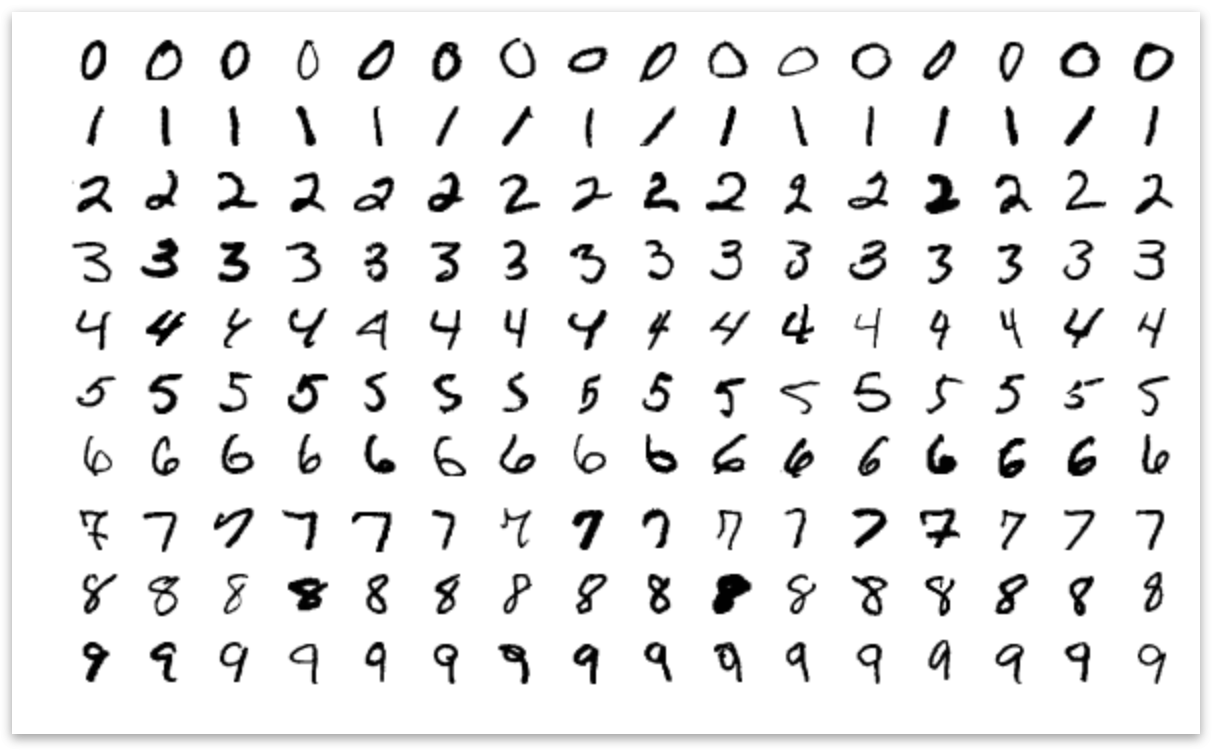
\includegraphics[width=0.5\textwidth]{Figures/Results/mnist.png}
  \caption[]{MNIST dataset example of handwritten digits.}
  \label{fig:mnist}
\end{figure}

The CNN was trained using the Radeon Vega Frontier Edition GPU, a top of the line graphics processor accelerator from AMD. This graphics card presents 8 levels of pairs of GPU Core frequency and voltage, Table \ref{tab:gpulevels}, that the GPU chooses in runtime accordingly to the temperature and power required, trying to maximize the performance. The GPU allows for the user definition of the frequency and voltage throw the ROCm System Management Interface - \textit{rocm-smi}. With it, a script was developed that performs undervoltage in steps of 10 mV on each of the 8 default voltage and frequency pairs. If the undervoltage is accepted by the software, the MNIST model is trained and after each run, the achieved accuracy is stored alongside the maximum power and average consumption, total energy consumed and the time that it took to execute the train.







\begin{figure}[!htb]
  \centering
  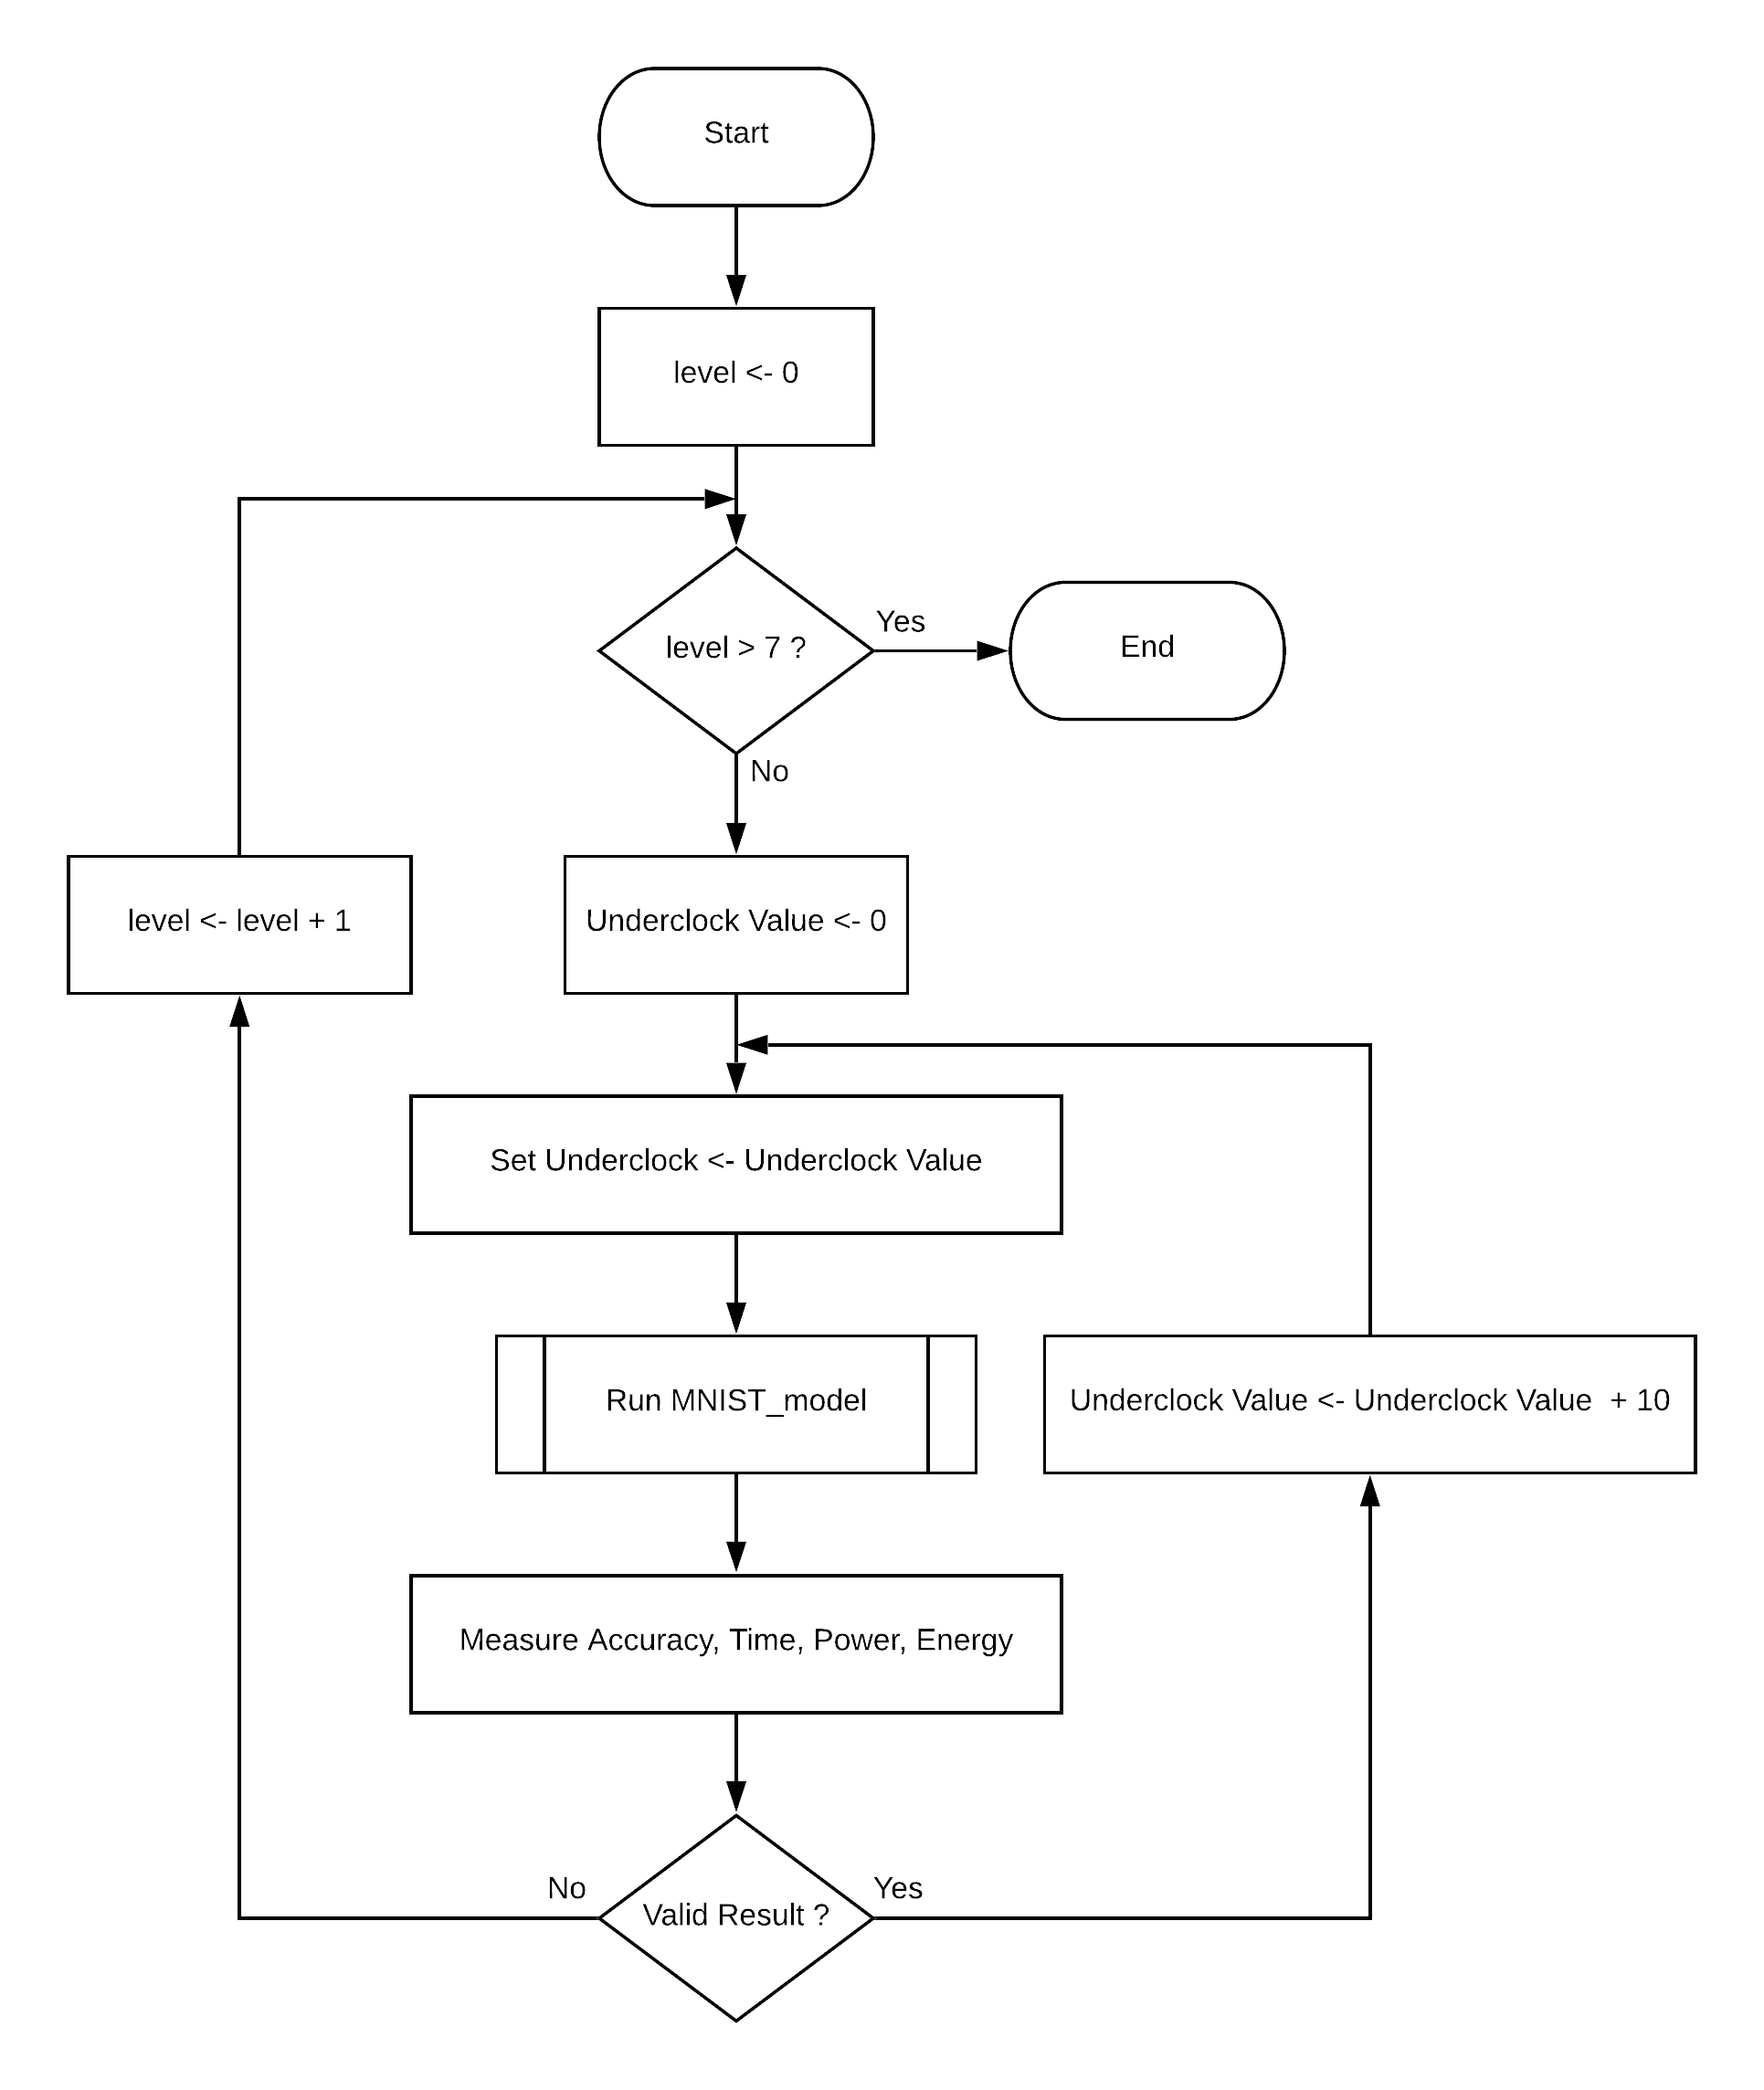
\includegraphics[width=0.75\textwidth]{Figures/Results/Underclock_Program.png}
  \caption[]{Flowchart of Automation Undervoltage Script.}
  \label{fig:undervoltage_program}
\end{figure}





\subsection{Preleminary Results}
\label{section:dvfseffects}

%%%%%%%%%%%%%%%%%%%%%%%%%%%%%%%%%%%%%%%%%%%%%%%%%%%%%%%%%%%%%%%%%%%%%%%%
\subsubsection{OverClock}
\label{section:underclock}

\subsubsection{UnderVoltage}




 % file "Thesis_Application.tex"
\cleardoublepage

%%%%%%%%%%%%%%%%%%%%%%%%%%%%%%%%%%%%%%%%%%%%%%%%%%%%%%%%%%%%%%%%%%%%%%%%
%                                                                      %
%     File: Thesis_Implementation.tex                                  %
%     Tex Master: Thesis.tex                                           %
%                                                                      %
%     Author: Francisco Mendes                                         %
%     Last modified :  28 Nov 2019                                     %
%                                                                      %
%%%%%%%%%%%%%%%%%%%%%%%%%%%%%%%%%%%%%%%%%%%%%%%%%%%%%%%%%%%%%%%%%%%%%%%%

\chapter{Proposal}
\label{chapter:implementation}
\begin{figure}[!htb]
  \centering
  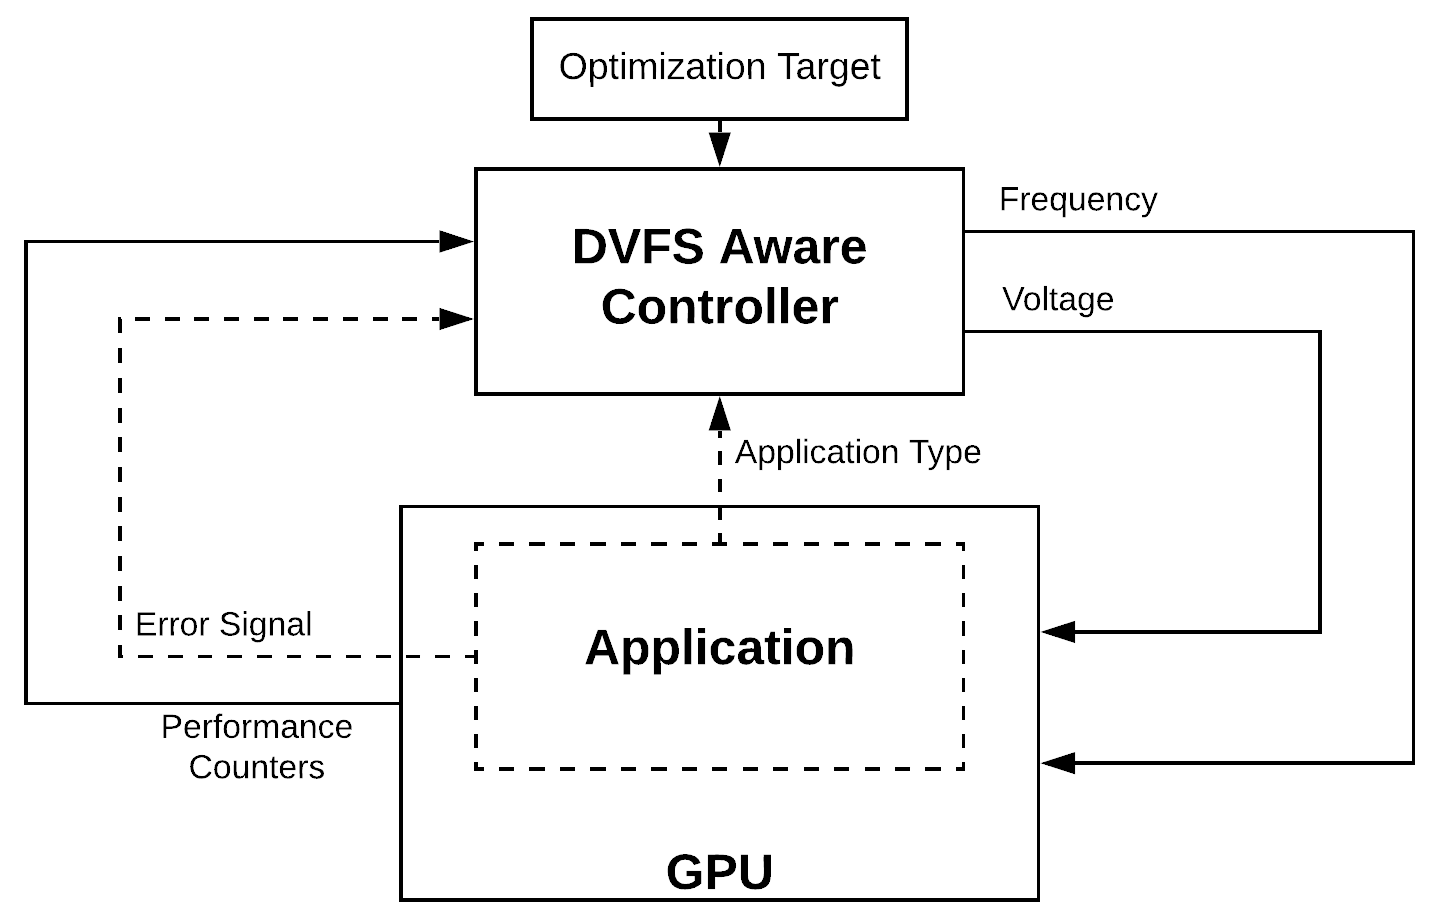
\includegraphics[width=0.75\textwidth]{Figures/Proposel/DVFS_Aware_Controller.png}
  \caption[Controller]{DVFS Aware Controller Block Diagram.}
  \label{fig:controlerDVFSaware}
\end{figure}

The main goal of this work is to designed and implement a GPU DVFS aware mechanism. This new mechanism will enforce non-conventional DVFS parameters to improve the energy efficiency of GPU devices, running deep learning applications. 

Two steps are required to acquire sufficient knowledge to design the controller. First, a characterization of the use of non-conventional DVFS parameters has to be performed for different workload scenarios, and second, a power and performance model has to be created. This chapter will start by providing an overview of how those two steps are going to be executed and what kinds of insights are expected to be uncovered. Then an overview of the GPU DVFS aware mechanism will be provided, connecting how do the previous points are connect, in the architecture of the solution. Finally, an overview of how the mechanism will be tested is described is presented.

The experimental work will be conducted on the Radeon Vega Frontier Edition presented in Chapter 2. This GPU provides the two necessary tools to both do the DVFS exploration and customization implementation through the profiling software - ROC-Profiler \cite{noauthor_rocm-developer-tools/rocprofiler_2019}, and tunning software - ROC-SMI \cite{noauthor_radeonopencompute/roc-smi_2019}.

\section{Non-convectional GPU DVFS characterization}

The objective of the characterization is to understand how the different workloads impact the voltage margin and how does performance and energy consumption relates to DVFS parameters. 

This part of the work will extend the work of Guerreiro \textit{et al.} in \cite{guerreiro_gpgpu_2018} \cite{guerreiro_modeling_2019} and Leng \textit{et al.} in \cite{leng_safe_2015}, by combining aggressive but safe voltage reduction with the
drawing of optimization curves, like the one of Figure \ref{fig:optcurves}. In this kind of plot, points of frequency/voltage are drawn, relating the performance achieved with the amount of energy spent. By using it, it is possible to optimize the DVFS settings for pure performance, energy efficiency or energy saving.

\begin{figure}[!htb]
  \centering
  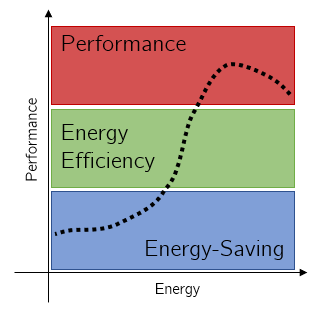
\includegraphics[width=0.3\textwidth]{Figures/Proposel/curves.png}
  \caption[Controller]{Example of optimization curve.}
  \label{fig:optcurves}
\end{figure}

The characterization will be done in two levels, first a fundamental analysis, using simple benchmarks, and at a higher level, using DNN primitives individually.

\subsection{Fundamental Analysis}
\label{sec:funAnali}
As stated in chapter 2, GPUs contain a significant voltage guardband to guarantee correct operation for all kinds of workloads and to be able to resist voltage noise. Using the benchmarks presented in Section \ref{sec:funAnal}, the size of these margins will be measured, first for each kind of benchmarks, and then to combinations of them, mimicking more complex workloads. This analysis will be performed by repeatedly running each benchmark at increasingly reduced voltage, and evaluating if the results being produced are the ones expected. When a benchmark is not able to be run at the indented under-voltage value, due to computation errors, or GPU crashes, the minimum voltage, $V_{min}$, is identified.

This analysis will allow an understanding of the impact that the activation and deactivation of the different GPU components cause on the voltage noise, the main contributing factor to the size of the voltage guardband.

The second part of the analysis is to create the optimization curves for each benchmark type and to comprehend what types of workloads have a dominant weight over $V_{min}$, performance and energy.


\subsection{DNN Primitives Analysis}
The insights of the fundamental analysis will help to guide the DNN primitive analysis and characterization. Here, the benchmarks proposed in Section \ref{sec:dnnPri} will be used to understand how to optimize the different layers of a complete DNN. 

On the preliminary work, Section 3.3, the $V_{min}$ was determined for a CNN; however, this results only indicates that there is a specific layer on that CNN that has the determined  $V_{min}$. The characterization of DVFS parameters in a per layer way allows for further optimizations of the DVFS to the running neural network.

\section{Power and Performance Model}
The second step to create the DVFS aware mechanism is to have a valid prediction model for power and performance. This mechanism will use the performance counters extracted from the runtime of the benchmarks from Section \ref{sec:funAnal} and ref{sec:dnnPri}, references for the type of application and user input of the desired optimization (performance, energy efficiency or energy saving) to predict $V_min$ and the best pair of frequency/voltage. Figure \ref{fig:model} exemplifies the block diagram of the power and performance model.

\begin{figure}[!htb]
  \centering
  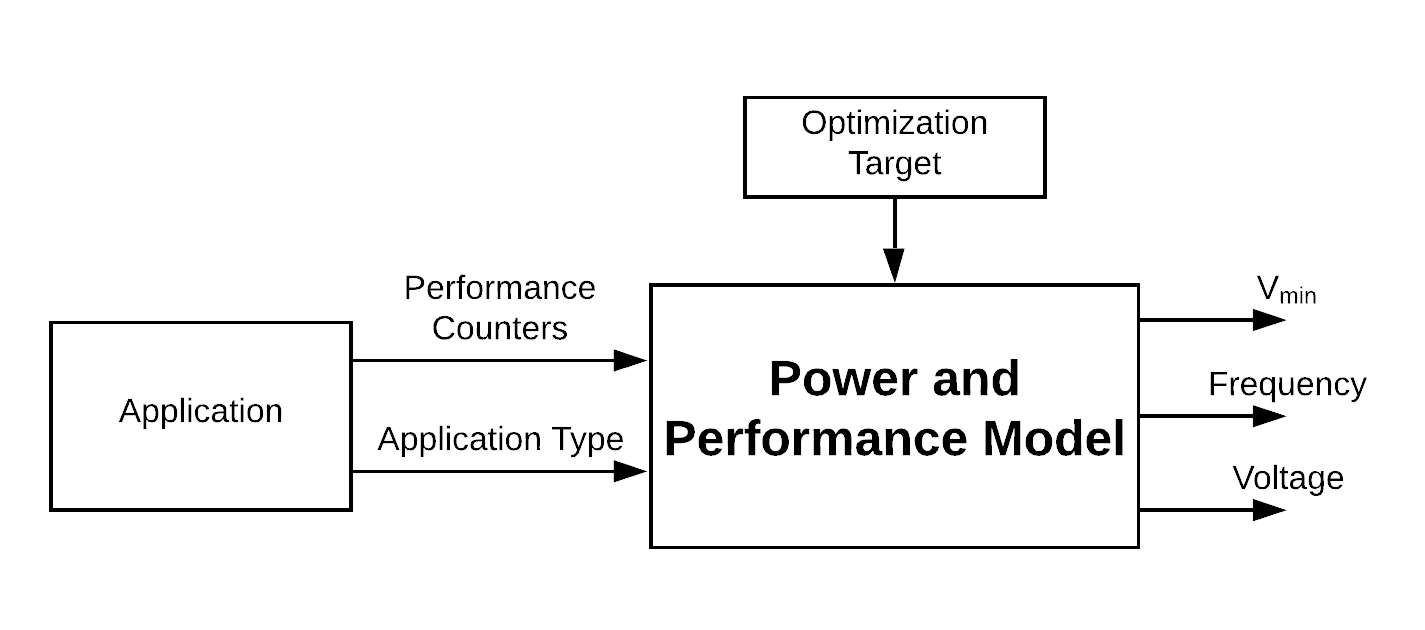
\includegraphics[width=0.8\textwidth]{Figures/Proposel/model.png}
  \caption[Controller]{Block Diagram of Power and Performance Model.}
  \label{fig:model}
\end{figure}. 

The profiling results from Section 4.1.1,  (performance counters values, performance, power and energy) will be used to train an artificial neural network (ANN) that will model the power and prediction. Following the approach of Song \textit{et al.} \cite{song_simplified_2013} and Guerreiro  \textit{et al.} \cite{guerreiro_modeling_2019}, the trained ANN should be able to correctly predict the best DVFS settings for both simple kernels, as well, for DNN primitives and full DNN layers from Section 4.1.2.

%%%%%%%%%%%%%%%%%%%%%%%%%%%%%%%%%%%%%%%%%%%%%%%%%%%%%%%%%%%%%%%%%%%%%%%%
\section{GPU DVFS Aware Mechanism}
\label{section:DVFSaware}

To design the controller, it is first necessary to extend the profiling application to support on-demand performance counters query and profiling of none C based applications. Since the deep learning libraries and applications used nowadays are developed in Python, a C static library will be developed, in order to have access to the performance counters values, at higher-level programming languages.

With an on-demand profiler, it is possible to construct a \textit{watch} application responsible for monitoring both the GPU and the deep learning application state. The \textit{watch} application will control the AMD DVFS mechanism, through the ROC-SMI interface, by providing the best frequency and voltage level for each performance level and by setting, depending on the DNN layer running, the most appropriated performance level, depending on the user optimization target (performance, energy efficiency or energy savings).



 % file "Thesis_Proposel.tex"
\cleardoublepage

%\input{Thesis_new_file} % add new .tex files for new chapters
% \cleardoublepage




% ----------------------------------------------------------------------
%  Bibliography
% ----------------------------------------------------------------------

% Add entry in the table of contents as chapter
\phantomsection
\addcontentsline{toc}{chapter}{\bibname}

% Include all references in .bib file, even non-cited ones...
%\nocite{*} % this should be used carefully because it is not correct!

% Produces the bibliography section when processed by BibTeX
%
% Bibliography style
% > entries ordered alphabetically
%\bibliographystyle{plain}
% > unsorted with entries appearing in the order in which the citations appear.
%\bibliographystyle{unsrt}
% > entries ordered alphabetically, with first names and names of journals and months abbreviated
%\bibliographystyle{abbrv}
% > entries ordered alphabetically, with reference markers based on authors' initials and publication year
%\bibliographystyle{alpha}
%
% Replacement bibliography styles provided by 'natbib' package
% (plainnat.bst, abbrvnat.bst, unsrtnat.bst )
% > entries ordered alphabetically
%\bibliographystyle{plainnat}
% > unsorted with entries appearing in the order in which the citations appear.
%\bibliographystyle{unsrtnat}
% > entries ordered alphabetically, with first names and names of journals and months abbreviated
%\bibliographystyle{abbrvnat} % <<<<< SELECT IF USING REFERENCES BY AUTHOR/YEAR
% > entries ordered alphabetically, with reference markers based on authors' initials and publication year
%\bibliographystyle{alpha}
%
% Custom bibliography style adapted from 'natbib' package
%   (based on http://tex.stackexchange.com/questions/5053/is-it-possible-to-get-unsrt-abbrv-bibliography)
%   (unsrtnat.bst + abbrvnat.bst -> abbrvunsrtnat.bst)
%   (original files copied from:
%   http://tug.ctan.org/macros/latex/contrib/natbib/abbrvnat.bst
%   http://tug.ctan.org/macros/latex/contrib/natbib/unsrtnat.bst
% > unsorted with entries appearing in the order in which the citations appear, with first names and names of journals and months abbreviated.
\bibliographystyle{abbrvunsrtnat} % <<<<< SELECT IF USING REFERENCES BY NUMBER (CITATION ORDER)

% External bibliography database file in the BibTeX format
\bibliography{references} % file "references.bib" //from zotero


% ----------------------------------------------------------------------
\end{document}
% ----------------------------------------------------------------------

